\documentclass[twoside]{book}

% Packages required by doxygen
\usepackage{calc}
\usepackage{doxygen}
\usepackage{graphicx}
\usepackage[utf8]{inputenc}
\usepackage{makeidx}
\usepackage{multicol}
\usepackage{multirow}
\usepackage{textcomp}
\usepackage[table]{xcolor}

% Font selection
\usepackage[T1]{fontenc}
\usepackage{mathptmx}
\usepackage[scaled=.90]{helvet}
\usepackage{courier}
\usepackage{amssymb}
\usepackage{sectsty}
\renewcommand{\familydefault}{\sfdefault}
\allsectionsfont{%
  \fontseries{bc}\selectfont%
  \color{darkgray}%
}
\renewcommand{\DoxyLabelFont}{%
  \fontseries{bc}\selectfont%
  \color{darkgray}%
}

% Page & text layout
\usepackage{geometry}
\geometry{%
  a4paper,%
  top=2.5cm,%
  bottom=2.5cm,%
  left=2.5cm,%
  right=2.5cm%
}
\tolerance=750
\hfuzz=15pt
\hbadness=750
\setlength{\emergencystretch}{15pt}
\setlength{\parindent}{0cm}
\setlength{\parskip}{0.2cm}
\makeatletter
\renewcommand{\paragraph}{%
  \@startsection{paragraph}{4}{0ex}{-1.0ex}{1.0ex}{%
    \normalfont\normalsize\bfseries\SS@parafont%
  }%
}
\renewcommand{\subparagraph}{%
  \@startsection{subparagraph}{5}{0ex}{-1.0ex}{1.0ex}{%
    \normalfont\normalsize\bfseries\SS@subparafont%
  }%
}
\makeatother

% Headers & footers
\usepackage{fancyhdr}
\pagestyle{fancyplain}
\fancyhead[LE]{\fancyplain{}{\bfseries\thepage}}
\fancyhead[CE]{\fancyplain{}{}}
\fancyhead[RE]{\fancyplain{}{\bfseries\leftmark}}
\fancyhead[LO]{\fancyplain{}{\bfseries\rightmark}}
\fancyhead[CO]{\fancyplain{}{}}
\fancyhead[RO]{\fancyplain{}{\bfseries\thepage}}
\fancyfoot[LE]{\fancyplain{}{}}
\fancyfoot[CE]{\fancyplain{}{}}
\fancyfoot[RE]{\fancyplain{}{\bfseries\scriptsize Generated on Fri May 29 2015 17\-:15\-:16 for My Project by Doxygen }}
\fancyfoot[LO]{\fancyplain{}{\bfseries\scriptsize Generated on Fri May 29 2015 17\-:15\-:16 for My Project by Doxygen }}
\fancyfoot[CO]{\fancyplain{}{}}
\fancyfoot[RO]{\fancyplain{}{}}
\renewcommand{\footrulewidth}{0.4pt}
\renewcommand{\chaptermark}[1]{%
  \markboth{#1}{}%
}
\renewcommand{\sectionmark}[1]{%
  \markright{\thesection\ #1}%
}

% Indices & bibliography
\usepackage{natbib}
\usepackage[titles]{tocloft}
\setcounter{tocdepth}{3}
\setcounter{secnumdepth}{5}
\makeindex

% Hyperlinks (required, but should be loaded last)
\usepackage{ifpdf}
\ifpdf
  \usepackage[pdftex,pagebackref=true]{hyperref}
\else
  \usepackage[ps2pdf,pagebackref=true]{hyperref}
\fi
\hypersetup{%
  colorlinks=true,%
  linkcolor=blue,%
  citecolor=blue,%
  unicode%
}

% Custom commands
\newcommand{\clearemptydoublepage}{%
  \newpage{\pagestyle{empty}\cleardoublepage}%
}


%===== C O N T E N T S =====

\begin{document}

% Titlepage & ToC
\hypersetup{pageanchor=false}
\pagenumbering{roman}
\begin{titlepage}
\vspace*{7cm}
\begin{center}%
{\Large My Project }\\
\vspace*{1cm}
{\large Generated by Doxygen 1.8.6}\\
\vspace*{0.5cm}
{\small Fri May 29 2015 17:15:16}\\
\end{center}
\end{titlepage}
\clearemptydoublepage
\tableofcontents
\clearemptydoublepage
\pagenumbering{arabic}
\hypersetup{pageanchor=true}

%--- Begin generated contents ---
\chapter{Main Page}
\label{index}\hypertarget{index}{}\begin{DoxyAuthor}{Author}
Bartłomiej Ankowski 
\end{DoxyAuthor}
\begin{DoxyDate}{Date}
16.\-04.\-2015 
\end{DoxyDate}
\begin{DoxyVersion}{Version}
0.\-3 \par

\end{DoxyVersion}
\hypertarget{index_Opis}{}\section{Programu}\label{index_Opis}

\chapter{Hierarchical Index}
\section{Class Hierarchy}
This inheritance list is sorted roughly, but not completely, alphabetically\-:\begin{DoxyCompactList}
\item \contentsline{section}{Czasomierz}{\pageref{class_czasomierz}}{}
\item \contentsline{section}{I\-Obserwator}{\pageref{class_i_obserwator}}{}
\begin{DoxyCompactList}
\item \contentsline{section}{Wyniki}{\pageref{class_wyniki}}{}
\end{DoxyCompactList}
\item \contentsline{section}{I\-Obserwowany}{\pageref{class_i_obserwowany}}{}
\begin{DoxyCompactList}
\item \contentsline{section}{Struktury\-Benchmark$<$ Typ $>$}{\pageref{class_struktury_benchmark}}{}
\end{DoxyCompactList}
\item \contentsline{section}{Itest}{\pageref{class_itest}}{}
\begin{DoxyCompactList}
\item \contentsline{section}{Graf$<$ Typ $>$}{\pageref{class_graf}}{}
\end{DoxyCompactList}
\item \contentsline{section}{Struktury$<$ Typ $>$}{\pageref{class_struktury}}{}
\begin{DoxyCompactList}
\item \contentsline{section}{Kolejka$<$ Typ $>$}{\pageref{class_kolejka}}{}
\item \contentsline{section}{Lista$<$ Typ $>$}{\pageref{class_lista}}{}
\item \contentsline{section}{Stos\-Tab$<$ Typ $>$}{\pageref{class_stos_tab}}{}
\end{DoxyCompactList}
\item \contentsline{section}{Kolejka$<$ Typ $>$\-:\-:Wezel}{\pageref{struct_kolejka_1_1_wezel}}{}
\item \contentsline{section}{Lista$<$ Typ $>$\-:\-:Wezel}{\pageref{struct_lista_1_1_wezel}}{}
\end{DoxyCompactList}

\chapter{Class Index}
\section{Class List}
Here are the classes, structs, unions and interfaces with brief descriptions\-:\begin{DoxyCompactList}
\item\contentsline{section}{\hyperlink{class_czasomierz}{Czasomierz} \\*Modeluje pojecie Czasomierza }{\pageref{class_czasomierz}}{}
\item\contentsline{section}{\hyperlink{class_graf}{Graf$<$ Typ $>$} \\*Modeluje pojecie grafu }{\pageref{class_graf}}{}
\item\contentsline{section}{\hyperlink{class_i_obserwator}{I\-Obserwator} \\*Modeluje pojecie interfejsu dla obserwatora }{\pageref{class_i_obserwator}}{}
\item\contentsline{section}{\hyperlink{class_i_obserwowany}{I\-Obserwowany} \\*Interfejs dla Obserwatora }{\pageref{class_i_obserwowany}}{}
\item\contentsline{section}{\hyperlink{class_itest}{Itest} \\*Modeluje pojecie Interfejsu Testujacego }{\pageref{class_itest}}{}
\item\contentsline{section}{\hyperlink{class_kolejka}{Kolejka$<$ Typ $>$} \\*Modeluje pojecie Kolejki }{\pageref{class_kolejka}}{}
\item\contentsline{section}{\hyperlink{class_lista}{Lista$<$ Typ $>$} }{\pageref{class_lista}}{}
\item\contentsline{section}{\hyperlink{class_stos_tab}{Stos\-Tab$<$ Typ $>$} }{\pageref{class_stos_tab}}{}
\item\contentsline{section}{\hyperlink{class_struktury}{Struktury$<$ Typ $>$} \\*Modeluje pojecie \hyperlink{class_struktury}{Struktury} danych, klasa bazowa dla Stosu,Kolejki i Listy,zarowno w implemenetacji wskaznikowej jak i tablicowej }{\pageref{class_struktury}}{}
\item\contentsline{section}{\hyperlink{class_struktury_benchmark}{Struktury\-Benchmark$<$ Typ $>$} }{\pageref{class_struktury_benchmark}}{}
\item\contentsline{section}{\hyperlink{struct_kolejka_1_1_wezel}{Kolejka$<$ Typ $>$\-::\-Wezel} }{\pageref{struct_kolejka_1_1_wezel}}{}
\item\contentsline{section}{\hyperlink{struct_lista_1_1_wezel}{Lista$<$ Typ $>$\-::\-Wezel} }{\pageref{struct_lista_1_1_wezel}}{}
\item\contentsline{section}{\hyperlink{class_wyniki}{Wyniki} }{\pageref{class_wyniki}}{}
\end{DoxyCompactList}

\chapter{File Index}
\section{File List}
Here is a list of all files with brief descriptions\-:\begin{DoxyCompactList}
\item\contentsline{section}{/home/bartolomeo/209255/prj/inc/\hyperlink{_czasomierz_8hh}{Czasomierz.\-hh} }{\pageref{_czasomierz_8hh}}{}
\item\contentsline{section}{/home/bartolomeo/209255/prj/inc/\hyperlink{_graf_8hh}{Graf.\-hh} }{\pageref{_graf_8hh}}{}
\item\contentsline{section}{/home/bartolomeo/209255/prj/inc/\hyperlink{_i_obserwator_8hh}{I\-Obserwator.\-hh} }{\pageref{_i_obserwator_8hh}}{}
\item\contentsline{section}{/home/bartolomeo/209255/prj/inc/\hyperlink{_i_obserwowany_8hh}{I\-Obserwowany.\-hh} }{\pageref{_i_obserwowany_8hh}}{}
\item\contentsline{section}{/home/bartolomeo/209255/prj/inc/\hyperlink{_itest_8hh}{Itest.\-hh} }{\pageref{_itest_8hh}}{}
\item\contentsline{section}{/home/bartolomeo/209255/prj/inc/\hyperlink{_kolejka_8hh}{Kolejka.\-hh} }{\pageref{_kolejka_8hh}}{}
\item\contentsline{section}{/home/bartolomeo/209255/prj/inc/\hyperlink{_lista_8hh}{Lista.\-hh} }{\pageref{_lista_8hh}}{}
\item\contentsline{section}{/home/bartolomeo/209255/prj/inc/\hyperlink{_stos_tab_8hh}{Stos\-Tab.\-hh} }{\pageref{_stos_tab_8hh}}{}
\item\contentsline{section}{/home/bartolomeo/209255/prj/inc/\hyperlink{_struktury_8hh}{Struktury.\-hh} }{\pageref{_struktury_8hh}}{}
\item\contentsline{section}{/home/bartolomeo/209255/prj/inc/\hyperlink{_struktury_benchmark_8hh}{Struktury\-Benchmark.\-hh} }{\pageref{_struktury_benchmark_8hh}}{}
\item\contentsline{section}{/home/bartolomeo/209255/prj/inc/\hyperlink{_wyniki_8hh}{Wyniki.\-hh} }{\pageref{_wyniki_8hh}}{}
\item\contentsline{section}{/home/bartolomeo/209255/prj/src/\hyperlink{_czasomierz_8cpp}{Czasomierz.\-cpp} }{\pageref{_czasomierz_8cpp}}{}
\item\contentsline{section}{/home/bartolomeo/209255/prj/src/\hyperlink{_graf_8cpp}{Graf.\-cpp} }{\pageref{_graf_8cpp}}{}
\item\contentsline{section}{/home/bartolomeo/209255/prj/src/\hyperlink{_main_8cpp}{Main.\-cpp} \\*Funkcja glowna programu }{\pageref{_main_8cpp}}{}
\item\contentsline{section}{/home/bartolomeo/209255/prj/src/\hyperlink{_wyniki_8cpp}{Wyniki.\-cpp} }{\pageref{_wyniki_8cpp}}{}
\end{DoxyCompactList}

\chapter{Class Documentation}
\hypertarget{class_czasomierz}{\section{Czasomierz Class Reference}
\label{class_czasomierz}\index{Czasomierz@{Czasomierz}}
}


Modeluje pojecie Czasomierza.  




{\ttfamily \#include $<$Czasomierz.\-hh$>$}

\subsection*{Public Member Functions}
\begin{DoxyCompactItemize}
\item 
\hyperlink{class_czasomierz_aa49ccbbc365ff5e54b41f4ec4d769038}{Czasomierz} ()
\begin{DoxyCompactList}\small\item\em Konstruktor obiektu. \end{DoxyCompactList}\item 
void \hyperlink{class_czasomierz_a26f594c73a3b382d1695f14a5682ca7c}{\-\_\-\-Rozpocznij\-Pomiar} ()
\begin{DoxyCompactList}\small\item\em Metoda zaczynajaca pomiar. \end{DoxyCompactList}\item 
void \hyperlink{class_czasomierz_a91e1a8e33b5e1eb7a5036eed57fb13a3}{\-\_\-\-Zakoncz\-Pomiar} ()
\begin{DoxyCompactList}\small\item\em Metoda konczaca pomiar. \end{DoxyCompactList}\item 
void \hyperlink{class_czasomierz_aecc4b89376b85367ab0e44fecb4ca6df}{\-\_\-\-Aktualizuj\-Czas} ()
\begin{DoxyCompactList}\small\item\em Metoda Aktualizujaca czas danej proby. \end{DoxyCompactList}\item 
long double \hyperlink{class_czasomierz_a80be3a3d837f8ca28e1a6bc2f231f0d7}{\-\_\-\-Czas\-Trwania} () const 
\begin{DoxyCompactList}\small\item\em Metoda zwracajaca calkowity czas Proby. \end{DoxyCompactList}\item 
void \hyperlink{class_czasomierz_a1f2c55e5be7f93f3db9b02eb5757cc78}{\-\_\-\-Reset} ()
\begin{DoxyCompactList}\small\item\em Metoda resetujaca \hyperlink{class_czasomierz}{Czasomierz}. \end{DoxyCompactList}\item 
bool \hyperlink{class_czasomierz_ab5977fad1080924fe85f70157de7b4db}{\-\_\-\-Status\-Pracy} () const 
\item 
double \hyperlink{class_czasomierz_a02353d27a6e73f00e41c4c0b40990d58}{\-\_\-\-Pojedynczy\-Pomiar} () const 
\begin{DoxyCompactList}\small\item\em Metoda zwracajaca czas pojedynczego pomiaru. \end{DoxyCompactList}\end{DoxyCompactItemize}
\subsection*{Private Attributes}
\begin{DoxyCompactItemize}
\item 
clock\-\_\-t \hyperlink{class_czasomierz_aba798db3d70227410bfafbb01a52d755}{\-\_\-\-Start}
\begin{DoxyCompactList}\small\item\em Pole klasy \hyperlink{class_czasomierz}{Czasomierz}. \end{DoxyCompactList}\item 
clock\-\_\-t \hyperlink{class_czasomierz_a1d791b2017e7f992a2206155982055af}{\-\_\-\-Koniec}
\begin{DoxyCompactList}\small\item\em Pole klasy \hyperlink{class_czasomierz}{Czasomierz}. \end{DoxyCompactList}\item 
long double \hyperlink{class_czasomierz_ae09344cf8ca5613cd557cb4fcf9aa046}{\-\_\-\-Aktualny}
\begin{DoxyCompactList}\small\item\em Pole klasy \hyperlink{class_czasomierz}{Czasomierz}. \end{DoxyCompactList}\item 
bool \hyperlink{class_czasomierz_a5eb9aa3fd9f0fb8af343f2865d490e64}{\-\_\-\-Status}
\begin{DoxyCompactList}\small\item\em Pole klasy \hyperlink{class_czasomierz}{Czasomierz}. \end{DoxyCompactList}\end{DoxyCompactItemize}


\subsection{Detailed Description}
Modeluje pojecie Czasomierza. 

Klasa ma za zadanie mierzyc czas wykonywania danego algorytmu oraz przechowywac informacje o srednich czasach pomiarow dla wybranej ilosci danych przy okreslonej liczbie powtorzen testu 

\subsection{Constructor \& Destructor Documentation}
\hypertarget{class_czasomierz_aa49ccbbc365ff5e54b41f4ec4d769038}{\index{Czasomierz@{Czasomierz}!Czasomierz@{Czasomierz}}
\index{Czasomierz@{Czasomierz}!Czasomierz@{Czasomierz}}
\subsubsection[{Czasomierz}]{\setlength{\rightskip}{0pt plus 5cm}Czasomierz\-::\-Czasomierz (
\begin{DoxyParamCaption}
{}
\end{DoxyParamCaption}
)}}\label{class_czasomierz_aa49ccbbc365ff5e54b41f4ec4d769038}


Konstruktor obiektu. 

Konstruktor klasy \hyperlink{class_czasomierz}{Czasomierz}, zerujacy wszystkie pola tej klasy 

\subsection{Member Function Documentation}
\hypertarget{class_czasomierz_aecc4b89376b85367ab0e44fecb4ca6df}{\index{Czasomierz@{Czasomierz}!\-\_\-\-Aktualizuj\-Czas@{\-\_\-\-Aktualizuj\-Czas}}
\index{\-\_\-\-Aktualizuj\-Czas@{\-\_\-\-Aktualizuj\-Czas}!Czasomierz@{Czasomierz}}
\subsubsection[{\-\_\-\-Aktualizuj\-Czas}]{\setlength{\rightskip}{0pt plus 5cm}void Czasomierz\-::\-\_\-\-Aktualizuj\-Czas (
\begin{DoxyParamCaption}
{}
\end{DoxyParamCaption}
)}}\label{class_czasomierz_aecc4b89376b85367ab0e44fecb4ca6df}


Metoda Aktualizujaca czas danej proby. 

Metoda ma za zadanie zaktualizowac czas danej proby, za sprawa dodadania do poprzedniej sumy pomiarow, czas ktory przypada na najnowszy pomiar \hypertarget{class_czasomierz_a80be3a3d837f8ca28e1a6bc2f231f0d7}{\index{Czasomierz@{Czasomierz}!\-\_\-\-Czas\-Trwania@{\-\_\-\-Czas\-Trwania}}
\index{\-\_\-\-Czas\-Trwania@{\-\_\-\-Czas\-Trwania}!Czasomierz@{Czasomierz}}
\subsubsection[{\-\_\-\-Czas\-Trwania}]{\setlength{\rightskip}{0pt plus 5cm}long double Czasomierz\-::\-\_\-\-Czas\-Trwania (
\begin{DoxyParamCaption}
{}
\end{DoxyParamCaption}
) const}}\label{class_czasomierz_a80be3a3d837f8ca28e1a6bc2f231f0d7}


Metoda zwracajaca calkowity czas Proby. 

Metoda ma za zadanie zwrocic calkowity czas przypadajacy na dana probe \hypertarget{class_czasomierz_a02353d27a6e73f00e41c4c0b40990d58}{\index{Czasomierz@{Czasomierz}!\-\_\-\-Pojedynczy\-Pomiar@{\-\_\-\-Pojedynczy\-Pomiar}}
\index{\-\_\-\-Pojedynczy\-Pomiar@{\-\_\-\-Pojedynczy\-Pomiar}!Czasomierz@{Czasomierz}}
\subsubsection[{\-\_\-\-Pojedynczy\-Pomiar}]{\setlength{\rightskip}{0pt plus 5cm}double Czasomierz\-::\-\_\-\-Pojedynczy\-Pomiar (
\begin{DoxyParamCaption}
{}
\end{DoxyParamCaption}
) const}}\label{class_czasomierz_a02353d27a6e73f00e41c4c0b40990d58}


Metoda zwracajaca czas pojedynczego pomiaru. 

Metoda ma za zadanie zwrocic czas trwania pojedynczego testu \hypertarget{class_czasomierz_a1f2c55e5be7f93f3db9b02eb5757cc78}{\index{Czasomierz@{Czasomierz}!\-\_\-\-Reset@{\-\_\-\-Reset}}
\index{\-\_\-\-Reset@{\-\_\-\-Reset}!Czasomierz@{Czasomierz}}
\subsubsection[{\-\_\-\-Reset}]{\setlength{\rightskip}{0pt plus 5cm}void Czasomierz\-::\-\_\-\-Reset (
\begin{DoxyParamCaption}
{}
\end{DoxyParamCaption}
)}}\label{class_czasomierz_a1f2c55e5be7f93f3db9b02eb5757cc78}


Metoda resetujaca \hyperlink{class_czasomierz}{Czasomierz}. 

Metoda ma za zadanie wyzerowac pola przechowujace informacje o czasie systemowym zapisanym na poczatku i na koncu pomiaru. Zmienia status czasomierza na wolny \hypertarget{class_czasomierz_a26f594c73a3b382d1695f14a5682ca7c}{\index{Czasomierz@{Czasomierz}!\-\_\-\-Rozpocznij\-Pomiar@{\-\_\-\-Rozpocznij\-Pomiar}}
\index{\-\_\-\-Rozpocznij\-Pomiar@{\-\_\-\-Rozpocznij\-Pomiar}!Czasomierz@{Czasomierz}}
\subsubsection[{\-\_\-\-Rozpocznij\-Pomiar}]{\setlength{\rightskip}{0pt plus 5cm}void Czasomierz\-::\-\_\-\-Rozpocznij\-Pomiar (
\begin{DoxyParamCaption}
{}
\end{DoxyParamCaption}
)}}\label{class_czasomierz_a26f594c73a3b382d1695f14a5682ca7c}


Metoda zaczynajaca pomiar. 

Metoda ma za zadanie odczytac czas systemowy w momencie jej wywolania i zapisania tej informacji w odpowiednim polu klasy. Zmienia rowniez status pracy czasomierza na zajety. \hypertarget{class_czasomierz_ab5977fad1080924fe85f70157de7b4db}{\index{Czasomierz@{Czasomierz}!\-\_\-\-Status\-Pracy@{\-\_\-\-Status\-Pracy}}
\index{\-\_\-\-Status\-Pracy@{\-\_\-\-Status\-Pracy}!Czasomierz@{Czasomierz}}
\subsubsection[{\-\_\-\-Status\-Pracy}]{\setlength{\rightskip}{0pt plus 5cm}bool Czasomierz\-::\-\_\-\-Status\-Pracy (
\begin{DoxyParamCaption}
{}
\end{DoxyParamCaption}
) const}}\label{class_czasomierz_ab5977fad1080924fe85f70157de7b4db}
informujaca o stanie czasomierza

Metoda ma za zadanie poinformowanie w jakim stanie znajduje sie obecnie czasomierz \hypertarget{class_czasomierz_a91e1a8e33b5e1eb7a5036eed57fb13a3}{\index{Czasomierz@{Czasomierz}!\-\_\-\-Zakoncz\-Pomiar@{\-\_\-\-Zakoncz\-Pomiar}}
\index{\-\_\-\-Zakoncz\-Pomiar@{\-\_\-\-Zakoncz\-Pomiar}!Czasomierz@{Czasomierz}}
\subsubsection[{\-\_\-\-Zakoncz\-Pomiar}]{\setlength{\rightskip}{0pt plus 5cm}void Czasomierz\-::\-\_\-\-Zakoncz\-Pomiar (
\begin{DoxyParamCaption}
{}
\end{DoxyParamCaption}
)}}\label{class_czasomierz_a91e1a8e33b5e1eb7a5036eed57fb13a3}


Metoda konczaca pomiar. 

Metoda ma za zadanie odczytac czas systemowy w momencie jej wywolania i zapisania tej informacji w odpowiednim polu klasy. Zmienia status pracy czasomierza na wolny 

\subsection{Member Data Documentation}
\hypertarget{class_czasomierz_ae09344cf8ca5613cd557cb4fcf9aa046}{\index{Czasomierz@{Czasomierz}!\-\_\-\-Aktualny@{\-\_\-\-Aktualny}}
\index{\-\_\-\-Aktualny@{\-\_\-\-Aktualny}!Czasomierz@{Czasomierz}}
\subsubsection[{\-\_\-\-Aktualny}]{\setlength{\rightskip}{0pt plus 5cm}long double Czasomierz\-::\-\_\-\-Aktualny\hspace{0.3cm}{\ttfamily [private]}}}\label{class_czasomierz_ae09344cf8ca5613cd557cb4fcf9aa046}


Pole klasy \hyperlink{class_czasomierz}{Czasomierz}. 

Pole przechowuje czas w ms, odpowiadajacy czasowi aktualnego pomiaru dla danej ilosci danych \hypertarget{class_czasomierz_a1d791b2017e7f992a2206155982055af}{\index{Czasomierz@{Czasomierz}!\-\_\-\-Koniec@{\-\_\-\-Koniec}}
\index{\-\_\-\-Koniec@{\-\_\-\-Koniec}!Czasomierz@{Czasomierz}}
\subsubsection[{\-\_\-\-Koniec}]{\setlength{\rightskip}{0pt plus 5cm}clock\-\_\-t Czasomierz\-::\-\_\-\-Koniec\hspace{0.3cm}{\ttfamily [private]}}}\label{class_czasomierz_a1d791b2017e7f992a2206155982055af}


Pole klasy \hyperlink{class_czasomierz}{Czasomierz}. 

Pole przechowuje informacje, ktora jest czas systemu w chwili zakonczenia pomiaru \hypertarget{class_czasomierz_aba798db3d70227410bfafbb01a52d755}{\index{Czasomierz@{Czasomierz}!\-\_\-\-Start@{\-\_\-\-Start}}
\index{\-\_\-\-Start@{\-\_\-\-Start}!Czasomierz@{Czasomierz}}
\subsubsection[{\-\_\-\-Start}]{\setlength{\rightskip}{0pt plus 5cm}clock\-\_\-t Czasomierz\-::\-\_\-\-Start\hspace{0.3cm}{\ttfamily [private]}}}\label{class_czasomierz_aba798db3d70227410bfafbb01a52d755}


Pole klasy \hyperlink{class_czasomierz}{Czasomierz}. 

Pole przechowuje informacje, ktora jest czas systemu w chwili uruchomienia Stopera \hypertarget{class_czasomierz_a5eb9aa3fd9f0fb8af343f2865d490e64}{\index{Czasomierz@{Czasomierz}!\-\_\-\-Status@{\-\_\-\-Status}}
\index{\-\_\-\-Status@{\-\_\-\-Status}!Czasomierz@{Czasomierz}}
\subsubsection[{\-\_\-\-Status}]{\setlength{\rightskip}{0pt plus 5cm}bool Czasomierz\-::\-\_\-\-Status\hspace{0.3cm}{\ttfamily [private]}}}\label{class_czasomierz_a5eb9aa3fd9f0fb8af343f2865d490e64}


Pole klasy \hyperlink{class_czasomierz}{Czasomierz}. 

Pole przechowuje informacje o stanie Czasomierza,tzn czy obecnie odmierza czas czy nie 

The documentation for this class was generated from the following files\-:\begin{DoxyCompactItemize}
\item 
/home/bartolomeo/209255/prj/inc/\hyperlink{_czasomierz_8hh}{Czasomierz.\-hh}\item 
/home/bartolomeo/209255/prj/src/\hyperlink{_czasomierz_8cpp}{Czasomierz.\-cpp}\end{DoxyCompactItemize}

\hypertarget{class_graf}{\section{Graf$<$ Typ $>$ Class Template Reference}
\label{class_graf}\index{Graf$<$ Typ $>$@{Graf$<$ Typ $>$}}
}


Modeluje pojecie grafu.  




{\ttfamily \#include $<$Graf.\-hh$>$}

Inheritance diagram for Graf$<$ Typ $>$\-:\begin{figure}[H]
\begin{center}
\leavevmode
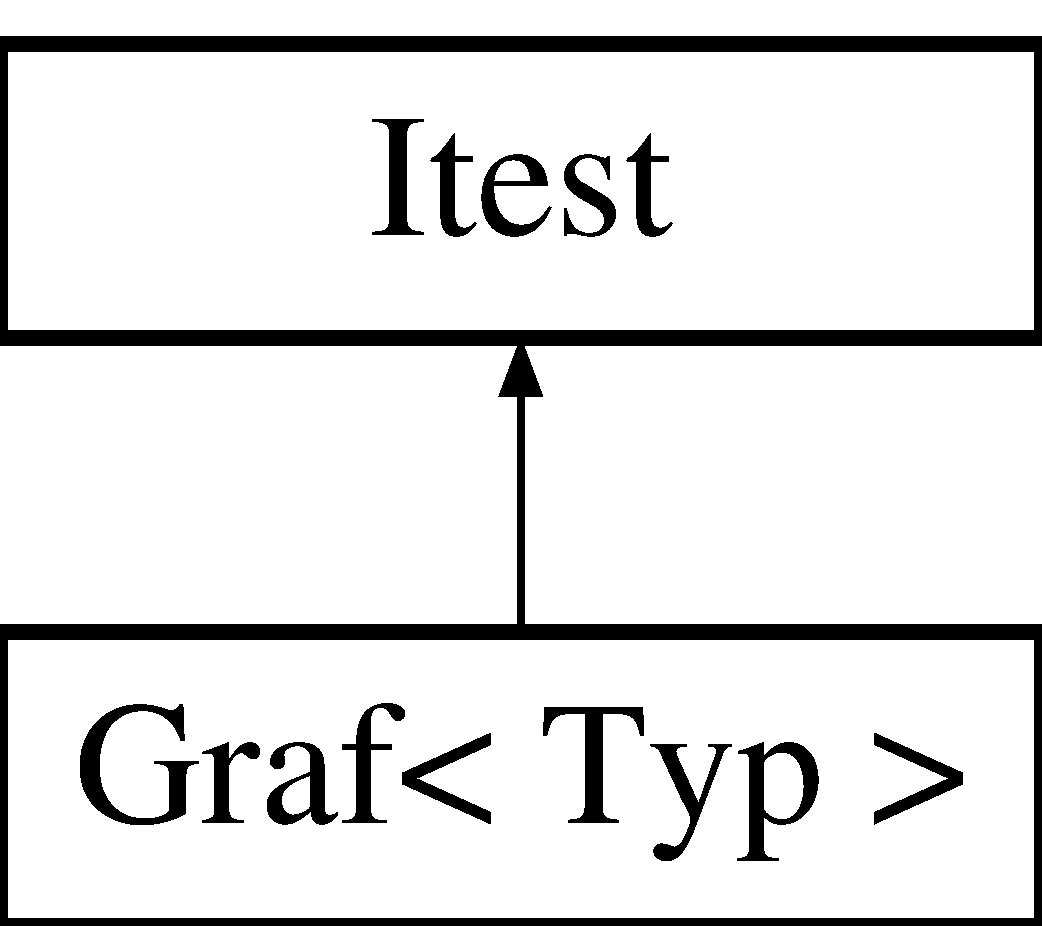
\includegraphics[height=2.000000cm]{class_graf}
\end{center}
\end{figure}
\subsection*{Public Member Functions}
\begin{DoxyCompactItemize}
\item 
void \hyperlink{class_graf_ac984753beb24de86d092a08b2cf844f1}{\-\_\-\-Wykonaj} (unsigned int n) const 
\begin{DoxyCompactList}\small\item\em Metoda wywolujaca testowany algorytm. \end{DoxyCompactList}\item 
void \hyperlink{class_graf_aaeb5adbe10a1a4fafdd0f62dac5ddbba}{\-\_\-\-Zwolnij} ()
\begin{DoxyCompactList}\small\item\em Metoda zwalniajaca pamiec. \end{DoxyCompactList}\item 
void \hyperlink{class_graf_adcb32f2e96badaa4d3cccd9de519f5b3}{\-\_\-\-Zaladuj} (unsigned int n)
\begin{DoxyCompactList}\small\item\em Metoda ladujaca dane. \end{DoxyCompactList}\item 
\hyperlink{class_graf_a95213c95392b1b99f83fcf89be540230}{Graf} (unsigned int n)
\begin{DoxyCompactList}\small\item\em Konstruktor obiektu. \end{DoxyCompactList}\item 
virtual \hyperlink{class_graf_ae738931dd17ef4e133757e76b960fc99}{$\sim$\-Graf} ()
\begin{DoxyCompactList}\small\item\em Destruktor obiektu. \end{DoxyCompactList}\item 
void \hyperlink{class_graf_a96466f767c7b1145421cf0c17a532449}{\-\_\-\-Dodaj\-Krawedz} (unsigned int i, unsigned int j)
\begin{DoxyCompactList}\small\item\em Metoda dodajaca Krawedz. \end{DoxyCompactList}\item 
void \hyperlink{class_graf_aea242f1a0b19b5768d516f92d224967f}{\-\_\-\-Usun\-Krawedz} (const unsigned int i, const unsigned int j)
\begin{DoxyCompactList}\small\item\em Metoda usuwajaca polaczenie. \end{DoxyCompactList}\item 
bool \hyperlink{class_graf_afa31377701d46bd692a6e430c6965d4b}{\-\_\-\-Czy\-Krawedz} (const unsigned int i, const unsigned int j) const 
\begin{DoxyCompactList}\small\item\em Metoda sprawdzajaca status polaczenia. \end{DoxyCompactList}\item 
void \hyperlink{class_graf_a1cef49af91f2d8b6f157e9dd06066d60}{B\-F\-S} (const int i, const int Szukany) const 
\begin{DoxyCompactList}\small\item\em Algorytm B\-F\-S. \end{DoxyCompactList}\item 
void \hyperlink{class_graf_a54e531a5abc04c9aaff81bd76aec5591}{D\-F\-S} (const int x, const int Wymagany) const 
\begin{DoxyCompactList}\small\item\em Algorytm B\-F\-S. \end{DoxyCompactList}\item 
void \hyperlink{class_graf_ae4fa759125334d0361226c4fa2dbf35e}{\-\_\-\-Dodaj\-Wartosc\-Wierzcholka} (const unsigned int indeks, const Typ Wartosc)
\begin{DoxyCompactList}\small\item\em Metoda dodajaca wartosc do danego wierzcholka. \end{DoxyCompactList}\item 
Typ \hyperlink{class_graf_a9198e4a7a0328ab5275713b4141fbb30}{\-\_\-\-Zwroc\-Wartosc\-Wierzcholka} (const unsigned int indeks) const 
\begin{DoxyCompactList}\small\item\em Metoda zwracajaca wartosc z wierzcholka. \end{DoxyCompactList}\item 
unsigned int \hyperlink{class_graf_adf42e78308217f1abbb79818abd04cdf}{\-\_\-\-Ilosc\-Krawedzi} () const 
\begin{DoxyCompactList}\small\item\em Metoda zwracaja ilsoc krawedzi. \end{DoxyCompactList}\end{DoxyCompactItemize}
\subsection*{Private Attributes}
\begin{DoxyCompactItemize}
\item 
unsigned int \hyperlink{class_graf_a43104495abdfb73304fccd5a6a2d89c2}{\-\_\-\-V}
\begin{DoxyCompactList}\small\item\em Pole Klasy \hyperlink{class_graf}{Graf}. \end{DoxyCompactList}\item 
unsigned int \hyperlink{class_graf_a7128b0f6457b5524673f93266648ae5b}{\-\_\-\-E}
\begin{DoxyCompactList}\small\item\em Pole klasy \hyperlink{class_graf}{Graf}. \end{DoxyCompactList}\item 
bool $\ast$$\ast$ \hyperlink{class_graf_a200828ae79157583b5e674cf8da6a134}{\-\_\-\-E\-Macierz}
\begin{DoxyCompactList}\small\item\em Pole klasy \hyperlink{class_graf}{Graf}. \end{DoxyCompactList}\item 
Typ $\ast$ \hyperlink{class_graf_a8f8bb580ab7939c3ca50cc759ec33a89}{\-\_\-\-V\-Macierz}
\begin{DoxyCompactList}\small\item\em Pole klasy \hyperlink{class_graf}{Graf}. \end{DoxyCompactList}\end{DoxyCompactItemize}


\subsection{Detailed Description}
\subsubsection*{template$<$class Typ$>$class Graf$<$ Typ $>$}

Modeluje pojecie grafu. 

Klasa modeluje pojecie Grafu, przedstawionego jako Macierz sasiedztw, ktora przechowuje informacje na temat polaczen miedzy wierzcholkami 

\subsection{Constructor \& Destructor Documentation}
\hypertarget{class_graf_a95213c95392b1b99f83fcf89be540230}{\index{Graf@{Graf}!Graf@{Graf}}
\index{Graf@{Graf}!Graf@{Graf}}
\subsubsection[{Graf}]{\setlength{\rightskip}{0pt plus 5cm}template$<$class Typ $>$ {\bf Graf}$<$ Typ $>$\-::{\bf Graf} (
\begin{DoxyParamCaption}
\item[{unsigned int}]{n}
\end{DoxyParamCaption}
)}}\label{class_graf_a95213c95392b1b99f83fcf89be540230}


Konstruktor obiektu. 

Konstruktor ma za zadanie zaalokowac pamiec potrzebna dla macerzy sasiedztw i wstepnie wypelnic ja wartosciami false


\begin{DoxyParams}[1]{Parameters}
\mbox{\tt in}  & {\em n} & -\/ wielkosc tworzenego grafu \\
\hline
\end{DoxyParams}
\hypertarget{class_graf_ae738931dd17ef4e133757e76b960fc99}{\index{Graf@{Graf}!$\sim$\-Graf@{$\sim$\-Graf}}
\index{$\sim$\-Graf@{$\sim$\-Graf}!Graf@{Graf}}
\subsubsection[{$\sim$\-Graf}]{\setlength{\rightskip}{0pt plus 5cm}template$<$class Typ $>$ {\bf Graf}$<$ Typ $>$\-::$\sim${\bf Graf} (
\begin{DoxyParamCaption}
{}
\end{DoxyParamCaption}
)\hspace{0.3cm}{\ttfamily [virtual]}}}\label{class_graf_ae738931dd17ef4e133757e76b960fc99}


Destruktor obiektu. 

Destruktor ma zazadanie uwolnic pamiec przeznaczona na realzizajcje grafu 

\subsection{Member Function Documentation}
\hypertarget{class_graf_afa31377701d46bd692a6e430c6965d4b}{\index{Graf@{Graf}!\-\_\-\-Czy\-Krawedz@{\-\_\-\-Czy\-Krawedz}}
\index{\-\_\-\-Czy\-Krawedz@{\-\_\-\-Czy\-Krawedz}!Graf@{Graf}}
\subsubsection[{\-\_\-\-Czy\-Krawedz}]{\setlength{\rightskip}{0pt plus 5cm}template$<$class Typ $>$ bool {\bf Graf}$<$ Typ $>$\-::\-\_\-\-Czy\-Krawedz (
\begin{DoxyParamCaption}
\item[{const unsigned int}]{i, }
\item[{const unsigned int}]{j}
\end{DoxyParamCaption}
) const}}\label{class_graf_afa31377701d46bd692a6e430c6965d4b}


Metoda sprawdzajaca status polaczenia. 

Metoda ma za zadanie sprawdzic status polaczenia miedzy wierzchokami zadanymi poprzez argument


\begin{DoxyParams}[1]{Parameters}
\mbox{\tt in}  & {\em i} & -\/ numer wierzcholka \\
\hline
\mbox{\tt in}  & {\em j} & -\/ numer wierzcholka \\
\hline
\end{DoxyParams}
\hypertarget{class_graf_a96466f767c7b1145421cf0c17a532449}{\index{Graf@{Graf}!\-\_\-\-Dodaj\-Krawedz@{\-\_\-\-Dodaj\-Krawedz}}
\index{\-\_\-\-Dodaj\-Krawedz@{\-\_\-\-Dodaj\-Krawedz}!Graf@{Graf}}
\subsubsection[{\-\_\-\-Dodaj\-Krawedz}]{\setlength{\rightskip}{0pt plus 5cm}template$<$class Typ $>$ void {\bf Graf}$<$ Typ $>$\-::\-\_\-\-Dodaj\-Krawedz (
\begin{DoxyParamCaption}
\item[{unsigned int}]{i, }
\item[{unsigned int}]{j}
\end{DoxyParamCaption}
)}}\label{class_graf_a96466f767c7b1145421cf0c17a532449}


Metoda dodajaca Krawedz. 

Metoda ma za zadanie zmienic status polaczen zadanych poprzez argument wierzcholkow na polaczony


\begin{DoxyParams}[1]{Parameters}
\mbox{\tt in}  & {\em i} & -\/ numer wierzcholka,ktory ma zostac polaczony z drugim argumentem \\
\hline
\mbox{\tt in}  & {\em j} & -\/ numer wierzcholka, ktory ma zostac polaczony z pierwszym argumentem \\
\hline
\end{DoxyParams}
\hypertarget{class_graf_ae4fa759125334d0361226c4fa2dbf35e}{\index{Graf@{Graf}!\-\_\-\-Dodaj\-Wartosc\-Wierzcholka@{\-\_\-\-Dodaj\-Wartosc\-Wierzcholka}}
\index{\-\_\-\-Dodaj\-Wartosc\-Wierzcholka@{\-\_\-\-Dodaj\-Wartosc\-Wierzcholka}!Graf@{Graf}}
\subsubsection[{\-\_\-\-Dodaj\-Wartosc\-Wierzcholka}]{\setlength{\rightskip}{0pt plus 5cm}template$<$class Typ $>$ void {\bf Graf}$<$ Typ $>$\-::\-\_\-\-Dodaj\-Wartosc\-Wierzcholka (
\begin{DoxyParamCaption}
\item[{const unsigned int}]{indeks, }
\item[{const Typ}]{Wartosc}
\end{DoxyParamCaption}
)}}\label{class_graf_ae4fa759125334d0361226c4fa2dbf35e}


Metoda dodajaca wartosc do danego wierzcholka. 

Metoda ma za zadanie dodac wartosc do danego wierzcholka


\begin{DoxyParams}[1]{Parameters}
\mbox{\tt in}  & {\em indeks} & -\/ Numer wierzcholka do ktorego ma zostac dodana wartosc \\
\hline
\mbox{\tt in}  & {\em Wartosc} & -\/ Wartosc,ktora ma zostac dodana do wierzcholka \\
\hline
\end{DoxyParams}
\hypertarget{class_graf_adf42e78308217f1abbb79818abd04cdf}{\index{Graf@{Graf}!\-\_\-\-Ilosc\-Krawedzi@{\-\_\-\-Ilosc\-Krawedzi}}
\index{\-\_\-\-Ilosc\-Krawedzi@{\-\_\-\-Ilosc\-Krawedzi}!Graf@{Graf}}
\subsubsection[{\-\_\-\-Ilosc\-Krawedzi}]{\setlength{\rightskip}{0pt plus 5cm}template$<$class Typ $>$ unsigned int {\bf Graf}$<$ Typ $>$\-::\-\_\-\-Ilosc\-Krawedzi (
\begin{DoxyParamCaption}
{}
\end{DoxyParamCaption}
) const}}\label{class_graf_adf42e78308217f1abbb79818abd04cdf}


Metoda zwracaja ilsoc krawedzi. 

Metoda ma za zadanie zwrocic ilosc krawedzi jaka zostala stworzona w zamodelowanym grafie

\begin{DoxyReturn}{Returns}
Ilosc krawedzi grafu 
\end{DoxyReturn}
\hypertarget{class_graf_aea242f1a0b19b5768d516f92d224967f}{\index{Graf@{Graf}!\-\_\-\-Usun\-Krawedz@{\-\_\-\-Usun\-Krawedz}}
\index{\-\_\-\-Usun\-Krawedz@{\-\_\-\-Usun\-Krawedz}!Graf@{Graf}}
\subsubsection[{\-\_\-\-Usun\-Krawedz}]{\setlength{\rightskip}{0pt plus 5cm}template$<$class Typ $>$ void {\bf Graf}$<$ Typ $>$\-::\-\_\-\-Usun\-Krawedz (
\begin{DoxyParamCaption}
\item[{const unsigned int}]{i, }
\item[{const unsigned int}]{j}
\end{DoxyParamCaption}
)}}\label{class_graf_aea242f1a0b19b5768d516f92d224967f}


Metoda usuwajaca polaczenie. 

Metoda ma zadanie usunac polaczenie miedzy wierzcholkami


\begin{DoxyParams}[1]{Parameters}
\mbox{\tt in}  & {\em i} & -\/ numer wierzcholka \\
\hline
\mbox{\tt in}  & {\em j} & -\/ numer wierzcholka \\
\hline
\end{DoxyParams}
\hypertarget{class_graf_ac984753beb24de86d092a08b2cf844f1}{\index{Graf@{Graf}!\-\_\-\-Wykonaj@{\-\_\-\-Wykonaj}}
\index{\-\_\-\-Wykonaj@{\-\_\-\-Wykonaj}!Graf@{Graf}}
\subsubsection[{\-\_\-\-Wykonaj}]{\setlength{\rightskip}{0pt plus 5cm}template$<$class Typ $>$ void {\bf Graf}$<$ Typ $>$\-::\-\_\-\-Wykonaj (
\begin{DoxyParamCaption}
\item[{unsigned int}]{n}
\end{DoxyParamCaption}
) const\hspace{0.3cm}{\ttfamily [virtual]}}}\label{class_graf_ac984753beb24de86d092a08b2cf844f1}


Metoda wywolujaca testowany algorytm. 

Metoda ma za zdanie wywolac zaimplementowany dla tej struktury danych algorytm


\begin{DoxyParams}[1]{Parameters}
\mbox{\tt in}  & {\em n} & -\/ Wielkosc problemu \\
\hline
\end{DoxyParams}


Implements \hyperlink{class_itest_a39d04d2e34c9d7e9606e3f987b683d5c}{Itest}.

\hypertarget{class_graf_adcb32f2e96badaa4d3cccd9de519f5b3}{\index{Graf@{Graf}!\-\_\-\-Zaladuj@{\-\_\-\-Zaladuj}}
\index{\-\_\-\-Zaladuj@{\-\_\-\-Zaladuj}!Graf@{Graf}}
\subsubsection[{\-\_\-\-Zaladuj}]{\setlength{\rightskip}{0pt plus 5cm}template$<$class Typ $>$ void {\bf Graf}$<$ Typ $>$\-::\-\_\-\-Zaladuj (
\begin{DoxyParamCaption}
\item[{unsigned int}]{n}
\end{DoxyParamCaption}
)\hspace{0.3cm}{\ttfamily [virtual]}}}\label{class_graf_adcb32f2e96badaa4d3cccd9de519f5b3}


Metoda ladujaca dane. 

Metoda ma za zadanie wypelnic macierz sasiedztw informacjami o typie polaczen miedzy wierzcholkami 

Implements \hyperlink{class_itest_a7565db7c0a4d736f218db9d0f5ceff7a}{Itest}.

\hypertarget{class_graf_aaeb5adbe10a1a4fafdd0f62dac5ddbba}{\index{Graf@{Graf}!\-\_\-\-Zwolnij@{\-\_\-\-Zwolnij}}
\index{\-\_\-\-Zwolnij@{\-\_\-\-Zwolnij}!Graf@{Graf}}
\subsubsection[{\-\_\-\-Zwolnij}]{\setlength{\rightskip}{0pt plus 5cm}template$<$class Typ $>$ void {\bf Graf}$<$ Typ $>$\-::\-\_\-\-Zwolnij (
\begin{DoxyParamCaption}
{}
\end{DoxyParamCaption}
)\hspace{0.3cm}{\ttfamily [virtual]}}}\label{class_graf_aaeb5adbe10a1a4fafdd0f62dac5ddbba}


Metoda zwalniajaca pamiec. 

Metoda ma za zadanie zwolnic pamiec, wykorzystana przez graf 
\begin{DoxyParams}[1]{Parameters}
\mbox{\tt in}  & {\em n} & -\/ Wielkosc problemu \\
\hline
\end{DoxyParams}


Implements \hyperlink{class_itest_a62ba16b48b1a40321cf8445db6a7b4f4}{Itest}.

\hypertarget{class_graf_a9198e4a7a0328ab5275713b4141fbb30}{\index{Graf@{Graf}!\-\_\-\-Zwroc\-Wartosc\-Wierzcholka@{\-\_\-\-Zwroc\-Wartosc\-Wierzcholka}}
\index{\-\_\-\-Zwroc\-Wartosc\-Wierzcholka@{\-\_\-\-Zwroc\-Wartosc\-Wierzcholka}!Graf@{Graf}}
\subsubsection[{\-\_\-\-Zwroc\-Wartosc\-Wierzcholka}]{\setlength{\rightskip}{0pt plus 5cm}template$<$class Typ $>$ Typ {\bf Graf}$<$ Typ $>$\-::\-\_\-\-Zwroc\-Wartosc\-Wierzcholka (
\begin{DoxyParamCaption}
\item[{const unsigned int}]{indeks}
\end{DoxyParamCaption}
) const}}\label{class_graf_a9198e4a7a0328ab5275713b4141fbb30}


Metoda zwracajaca wartosc z wierzcholka. 

Metoda ma za zadanie zwrocic wartosc z danego wierzcholka


\begin{DoxyParams}[1]{Parameters}
\mbox{\tt in}  & {\em indeks} & -\/ Indeks wierzcholka z ktorego ma zostac odczytana wartosc \\
\hline
\end{DoxyParams}
\hypertarget{class_graf_a1cef49af91f2d8b6f157e9dd06066d60}{\index{Graf@{Graf}!B\-F\-S@{B\-F\-S}}
\index{B\-F\-S@{B\-F\-S}!Graf@{Graf}}
\subsubsection[{B\-F\-S}]{\setlength{\rightskip}{0pt plus 5cm}template$<$class Typ $>$ void {\bf Graf}$<$ Typ $>$\-::B\-F\-S (
\begin{DoxyParamCaption}
\item[{const int}]{i, }
\item[{const int}]{Szukany}
\end{DoxyParamCaption}
) const}}\label{class_graf_a1cef49af91f2d8b6f157e9dd06066d60}


Algorytm B\-F\-S. 

Implemetacja algorytmu przechodzenia grafu wszerz, polegajacego na przechodzeniu grafu od zadanego wierzcholka i odwiedzeniu wszystkich dostepnych z niego wierzcholkow.\-Rezultatem jest drzewo przeszukiwania wszerz o korzeniu rownemu wierzcholkowi od ktorego rozpoczely sie poszukiwania


\begin{DoxyParams}[1]{Parameters}
\mbox{\tt in}  & {\em i} & -\/ Poczatkowy wierzcholek \\
\hline
\mbox{\tt in}  & {\em Szukany} & -\/ Wierzcholek koncowy \\
\hline
\end{DoxyParams}
\hypertarget{class_graf_a54e531a5abc04c9aaff81bd76aec5591}{\index{Graf@{Graf}!D\-F\-S@{D\-F\-S}}
\index{D\-F\-S@{D\-F\-S}!Graf@{Graf}}
\subsubsection[{D\-F\-S}]{\setlength{\rightskip}{0pt plus 5cm}template$<$class Typ $>$ void {\bf Graf}$<$ Typ $>$\-::D\-F\-S (
\begin{DoxyParamCaption}
\item[{const int}]{x, }
\item[{const int}]{Wymagany}
\end{DoxyParamCaption}
) const}}\label{class_graf_a54e531a5abc04c9aaff81bd76aec5591}


Algorytm B\-F\-S. 

Implementacja przechodzenia grafu w glab, polegajaca na badaniu wszystkich krawedzi wychodzacych z podanego wierzcholka. Po zbadaniu wszytskich krawedzi wychodzacych z danego wierzcholka algorytm powraca do wierzcholka z ktorego dany wierzcholek zostal odwiedzony


\begin{DoxyParams}[1]{Parameters}
\mbox{\tt in}  & {\em i} & -\/ Wierzcholek od ktorego zaczyna sie przechodzenie \\
\hline
\mbox{\tt in}  & {\em Szukany} & -\/ Wierzcholek na ktorym zakonczone zostaje przechodzenie grafu \\
\hline
\end{DoxyParams}


\subsection{Member Data Documentation}
\hypertarget{class_graf_a7128b0f6457b5524673f93266648ae5b}{\index{Graf@{Graf}!\-\_\-\-E@{\-\_\-\-E}}
\index{\-\_\-\-E@{\-\_\-\-E}!Graf@{Graf}}
\subsubsection[{\-\_\-\-E}]{\setlength{\rightskip}{0pt plus 5cm}template$<$class Typ $>$ unsigned int {\bf Graf}$<$ Typ $>$\-::\-\_\-\-E\hspace{0.3cm}{\ttfamily [private]}}}\label{class_graf_a7128b0f6457b5524673f93266648ae5b}


Pole klasy \hyperlink{class_graf}{Graf}. 

Pole zawiera informacje o ilosci krawedzi \hypertarget{class_graf_a200828ae79157583b5e674cf8da6a134}{\index{Graf@{Graf}!\-\_\-\-E\-Macierz@{\-\_\-\-E\-Macierz}}
\index{\-\_\-\-E\-Macierz@{\-\_\-\-E\-Macierz}!Graf@{Graf}}
\subsubsection[{\-\_\-\-E\-Macierz}]{\setlength{\rightskip}{0pt plus 5cm}template$<$class Typ $>$ bool$\ast$$\ast$ {\bf Graf}$<$ Typ $>$\-::\-\_\-\-E\-Macierz\hspace{0.3cm}{\ttfamily [private]}}}\label{class_graf_a200828ae79157583b5e674cf8da6a134}


Pole klasy \hyperlink{class_graf}{Graf}. 

Pole zawiera informace o polaczeniach miedzy wierzcholkami w grafie \hypertarget{class_graf_a43104495abdfb73304fccd5a6a2d89c2}{\index{Graf@{Graf}!\-\_\-\-V@{\-\_\-\-V}}
\index{\-\_\-\-V@{\-\_\-\-V}!Graf@{Graf}}
\subsubsection[{\-\_\-\-V}]{\setlength{\rightskip}{0pt plus 5cm}template$<$class Typ $>$ unsigned int {\bf Graf}$<$ Typ $>$\-::\-\_\-\-V\hspace{0.3cm}{\ttfamily [private]}}}\label{class_graf_a43104495abdfb73304fccd5a6a2d89c2}


Pole Klasy \hyperlink{class_graf}{Graf}. 

Pole zawiera informacje o ilosci wierzcholkow \hypertarget{class_graf_a8f8bb580ab7939c3ca50cc759ec33a89}{\index{Graf@{Graf}!\-\_\-\-V\-Macierz@{\-\_\-\-V\-Macierz}}
\index{\-\_\-\-V\-Macierz@{\-\_\-\-V\-Macierz}!Graf@{Graf}}
\subsubsection[{\-\_\-\-V\-Macierz}]{\setlength{\rightskip}{0pt plus 5cm}template$<$class Typ $>$ Typ$\ast$ {\bf Graf}$<$ Typ $>$\-::\-\_\-\-V\-Macierz\hspace{0.3cm}{\ttfamily [private]}}}\label{class_graf_a8f8bb580ab7939c3ca50cc759ec33a89}


Pole klasy \hyperlink{class_graf}{Graf}. 

Pole przechowuje informacje zapisana w danym wierzcholku 

The documentation for this class was generated from the following files\-:\begin{DoxyCompactItemize}
\item 
/home/bartolomeo/209255/prj/inc/\hyperlink{_graf_8hh}{Graf.\-hh}\item 
/home/bartolomeo/209255/prj/src/\hyperlink{_graf_8cpp}{Graf.\-cpp}\end{DoxyCompactItemize}

\hypertarget{class_i_obserwator}{\section{I\-Obserwator Class Reference}
\label{class_i_obserwator}\index{I\-Obserwator@{I\-Obserwator}}
}


Modeluje pojecie interfejsu dla obserwatora.  




{\ttfamily \#include $<$I\-Obserwator.\-hh$>$}

Inheritance diagram for I\-Obserwator\-:\begin{figure}[H]
\begin{center}
\leavevmode
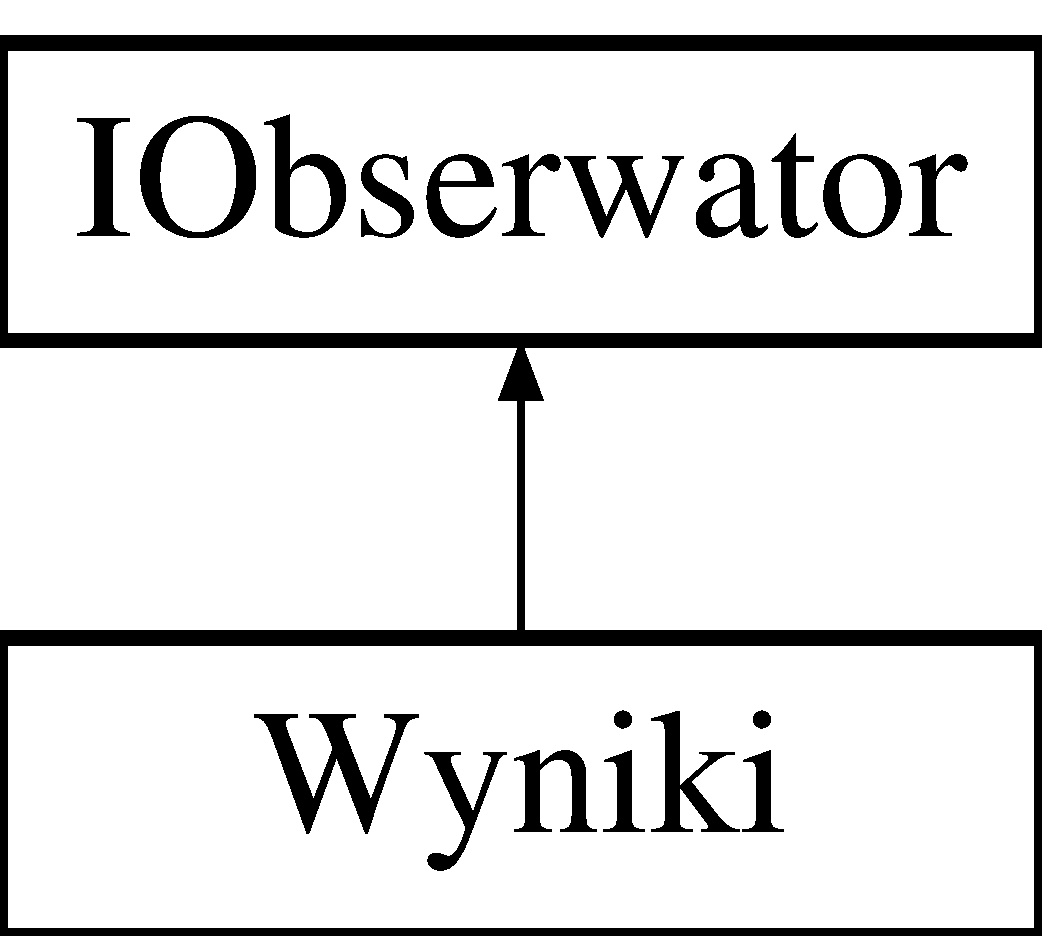
\includegraphics[height=2.000000cm]{class_i_obserwator}
\end{center}
\end{figure}
\subsection*{Public Member Functions}
\begin{DoxyCompactItemize}
\item 
virtual void \hyperlink{class_i_obserwator_ab01d64a94e127100951aa287d4d2275f}{\-\_\-\-Aktualizuj} ()=0
\begin{DoxyCompactList}\small\item\em Metoda Aktualizujaca stan. \end{DoxyCompactList}\end{DoxyCompactItemize}


\subsection{Detailed Description}
Modeluje pojecie interfejsu dla obserwatora. 

Klasa ta modeluje interfejs dla obiektu ktory bedzie obserwatorem 

\subsection{Member Function Documentation}
\hypertarget{class_i_obserwator_ab01d64a94e127100951aa287d4d2275f}{\index{I\-Obserwator@{I\-Obserwator}!\-\_\-\-Aktualizuj@{\-\_\-\-Aktualizuj}}
\index{\-\_\-\-Aktualizuj@{\-\_\-\-Aktualizuj}!IObserwator@{I\-Obserwator}}
\subsubsection[{\-\_\-\-Aktualizuj}]{\setlength{\rightskip}{0pt plus 5cm}virtual void I\-Obserwator\-::\-\_\-\-Aktualizuj (
\begin{DoxyParamCaption}
{}
\end{DoxyParamCaption}
)\hspace{0.3cm}{\ttfamily [pure virtual]}}}\label{class_i_obserwator_ab01d64a94e127100951aa287d4d2275f}


Metoda Aktualizujaca stan. 

Metoda ma za zadanie poinformowac o zmianach w obiekcie ktory jest obserwowany 

Implemented in \hyperlink{class_wyniki_a4014236438f62cfd90c03de49ea38e5f}{Wyniki}.



The documentation for this class was generated from the following file\-:\begin{DoxyCompactItemize}
\item 
/home/bartolomeo/209255/prj/inc/\hyperlink{_i_obserwator_8hh}{I\-Obserwator.\-hh}\end{DoxyCompactItemize}

\hypertarget{class_i_obserwowany}{\section{I\-Obserwowany Class Reference}
\label{class_i_obserwowany}\index{I\-Obserwowany@{I\-Obserwowany}}
}


Interfejs dla Obserwatora.  




{\ttfamily \#include $<$I\-Obserwowany.\-hh$>$}

Inheritance diagram for I\-Obserwowany\-:\begin{figure}[H]
\begin{center}
\leavevmode
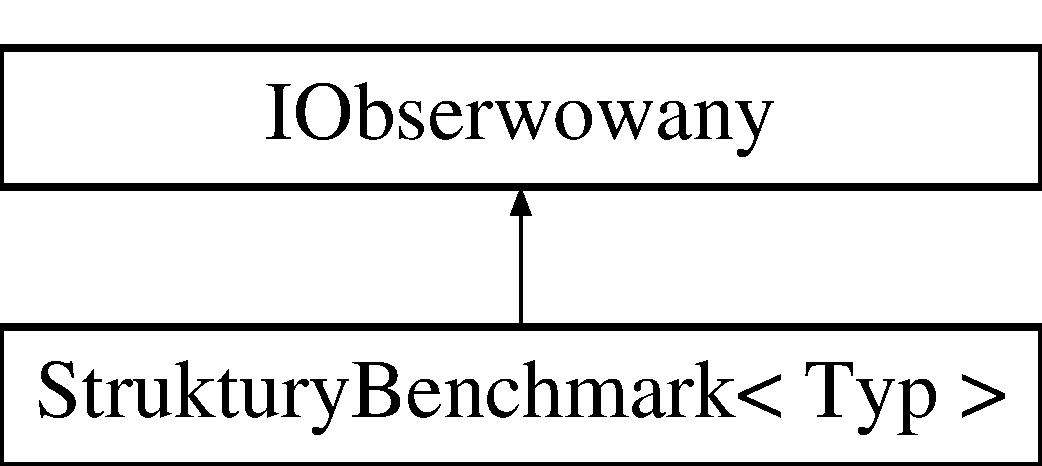
\includegraphics[height=2.000000cm]{class_i_obserwowany}
\end{center}
\end{figure}
\subsection*{Protected Member Functions}
\begin{DoxyCompactItemize}
\item 
virtual void \hyperlink{class_i_obserwowany_a3e7c49a1b168ed5a3f84bd0c5ae27513}{\-\_\-\-Dodaj\-Obserwator} (\hyperlink{class_i_obserwator}{I\-Obserwator} $\ast$O)=0
\begin{DoxyCompactList}\small\item\em Metoda dodajaca obserwator. \end{DoxyCompactList}\item 
virtual void \hyperlink{class_i_obserwowany_a6e91b84d0502f038d287152a5d860aff}{\-\_\-\-Usun\-Obserwator} (\hyperlink{class_i_obserwator}{I\-Obserwator} $\ast$O)=0
\begin{DoxyCompactList}\small\item\em Metoda usuwajaca obserwator. \end{DoxyCompactList}\item 
virtual void \hyperlink{class_i_obserwowany_addbe1bee0cae92b0c1348b2c6d0b525c}{\-\_\-\-Powiadom\-Obserwatorow} ()=0
\begin{DoxyCompactList}\small\item\em Metoda informujaca obserwatorow. \end{DoxyCompactList}\end{DoxyCompactItemize}


\subsection{Detailed Description}
Interfejs dla Obserwatora. 

Klasa modeluje pojecie abstrakcyjnego interfejsu dla klasy bedacej obiektem obserwowanym 

\subsection{Member Function Documentation}
\hypertarget{class_i_obserwowany_a3e7c49a1b168ed5a3f84bd0c5ae27513}{\index{I\-Obserwowany@{I\-Obserwowany}!\-\_\-\-Dodaj\-Obserwator@{\-\_\-\-Dodaj\-Obserwator}}
\index{\-\_\-\-Dodaj\-Obserwator@{\-\_\-\-Dodaj\-Obserwator}!IObserwowany@{I\-Obserwowany}}
\subsubsection[{\-\_\-\-Dodaj\-Obserwator}]{\setlength{\rightskip}{0pt plus 5cm}virtual void I\-Obserwowany\-::\-\_\-\-Dodaj\-Obserwator (
\begin{DoxyParamCaption}
\item[{{\bf I\-Obserwator} $\ast$}]{O}
\end{DoxyParamCaption}
)\hspace{0.3cm}{\ttfamily [protected]}, {\ttfamily [pure virtual]}}}\label{class_i_obserwowany_a3e7c49a1b168ed5a3f84bd0c5ae27513}


Metoda dodajaca obserwator. 

Metoda ma za zadanie dodac nowego obserwatora do listy obserwatorow danego obiektu


\begin{DoxyParams}[1]{Parameters}
\mbox{\tt in}  & {\em O} & -\/ wskaznik na dodawany obserwator \\
\hline
\end{DoxyParams}


Implemented in \hyperlink{class_struktury_benchmark_a63247cc5616565e429f5abd09d887630}{Struktury\-Benchmark$<$ Typ $>$}.

\hypertarget{class_i_obserwowany_addbe1bee0cae92b0c1348b2c6d0b525c}{\index{I\-Obserwowany@{I\-Obserwowany}!\-\_\-\-Powiadom\-Obserwatorow@{\-\_\-\-Powiadom\-Obserwatorow}}
\index{\-\_\-\-Powiadom\-Obserwatorow@{\-\_\-\-Powiadom\-Obserwatorow}!IObserwowany@{I\-Obserwowany}}
\subsubsection[{\-\_\-\-Powiadom\-Obserwatorow}]{\setlength{\rightskip}{0pt plus 5cm}virtual void I\-Obserwowany\-::\-\_\-\-Powiadom\-Obserwatorow (
\begin{DoxyParamCaption}
{}
\end{DoxyParamCaption}
)\hspace{0.3cm}{\ttfamily [protected]}, {\ttfamily [pure virtual]}}}\label{class_i_obserwowany_addbe1bee0cae92b0c1348b2c6d0b525c}


Metoda informujaca obserwatorow. 

Metoda ma za zadanie poinformowac wszystkich obserwatorow o zmianach, ktore sa istotne dla nich, jakie zostaly wykonane na obiekcie obserwowanym 

Implemented in \hyperlink{class_struktury_benchmark_af5aa09efcf9a1727e0868930b97ede49}{Struktury\-Benchmark$<$ Typ $>$}.

\hypertarget{class_i_obserwowany_a6e91b84d0502f038d287152a5d860aff}{\index{I\-Obserwowany@{I\-Obserwowany}!\-\_\-\-Usun\-Obserwator@{\-\_\-\-Usun\-Obserwator}}
\index{\-\_\-\-Usun\-Obserwator@{\-\_\-\-Usun\-Obserwator}!IObserwowany@{I\-Obserwowany}}
\subsubsection[{\-\_\-\-Usun\-Obserwator}]{\setlength{\rightskip}{0pt plus 5cm}virtual void I\-Obserwowany\-::\-\_\-\-Usun\-Obserwator (
\begin{DoxyParamCaption}
\item[{{\bf I\-Obserwator} $\ast$}]{O}
\end{DoxyParamCaption}
)\hspace{0.3cm}{\ttfamily [protected]}, {\ttfamily [pure virtual]}}}\label{class_i_obserwowany_a6e91b84d0502f038d287152a5d860aff}


Metoda usuwajaca obserwator. 

Metoda ma za zadanei usunac zadanego poprzez argument obserwatora z listy obserwatorow danego obiektu


\begin{DoxyParams}[1]{Parameters}
\mbox{\tt in}  & {\em O} & -\/ wskaznik na obserwator,ktory ma zostac usuniety \\
\hline
\end{DoxyParams}


Implemented in \hyperlink{class_struktury_benchmark_af08fe671ed7528428ffcb8a4daf65197}{Struktury\-Benchmark$<$ Typ $>$}.



The documentation for this class was generated from the following file\-:\begin{DoxyCompactItemize}
\item 
/home/bartolomeo/209255/prj/inc/\hyperlink{_i_obserwowany_8hh}{I\-Obserwowany.\-hh}\end{DoxyCompactItemize}

\hypertarget{class_itest}{\section{Itest Class Reference}
\label{class_itest}\index{Itest@{Itest}}
}


Modeluje pojecie Interfejsu Testujacego.  




{\ttfamily \#include $<$Itest.\-hh$>$}

Inheritance diagram for Itest\-:\begin{figure}[H]
\begin{center}
\leavevmode
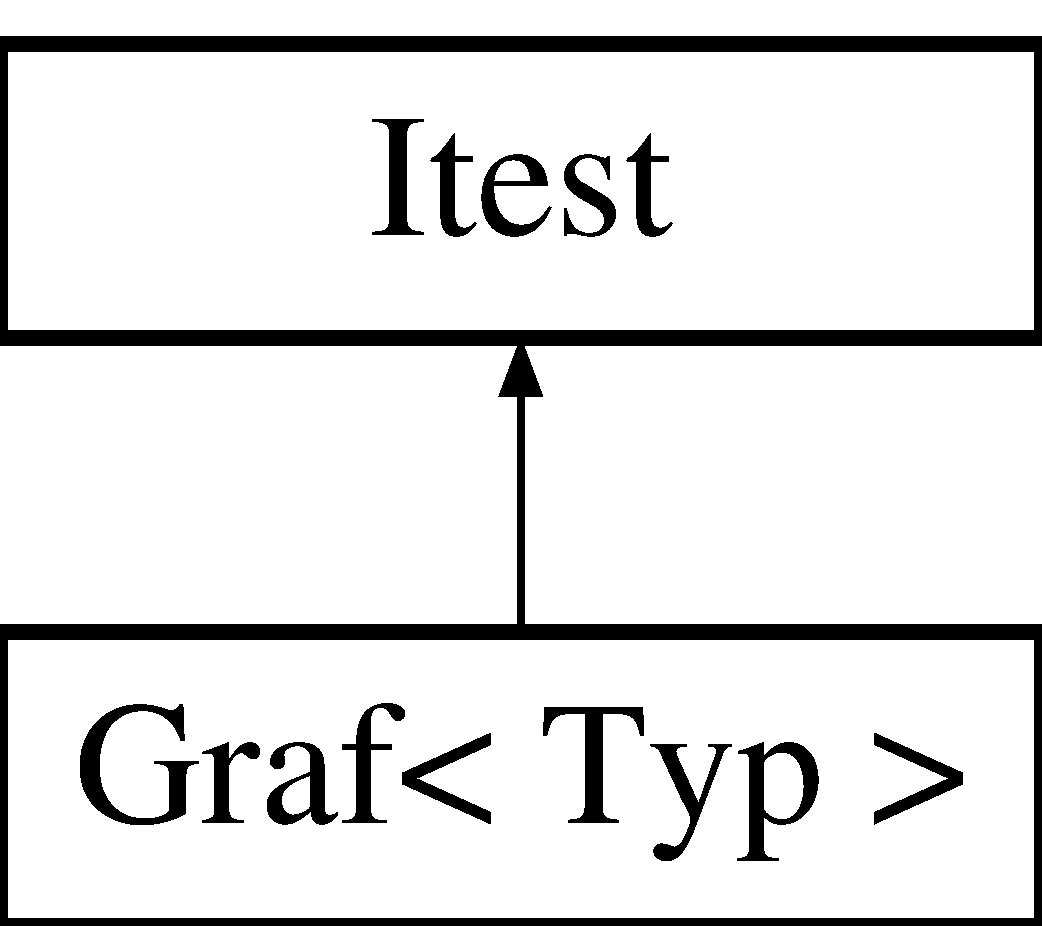
\includegraphics[height=2.000000cm]{class_itest}
\end{center}
\end{figure}
\subsection*{Public Member Functions}
\begin{DoxyCompactItemize}
\item 
virtual void \hyperlink{class_itest_a39d04d2e34c9d7e9606e3f987b683d5c}{\-\_\-\-Wykonaj} (unsigned int n) const =0
\begin{DoxyCompactList}\small\item\em Metoda Wywolujaca pojedyncza operacje. \end{DoxyCompactList}\item 
virtual void \hyperlink{class_itest_a62ba16b48b1a40321cf8445db6a7b4f4}{\-\_\-\-Zwolnij} ()=0
\begin{DoxyCompactList}\small\item\em Metoda zwalniajaca pamiec. \end{DoxyCompactList}\item 
virtual void \hyperlink{class_itest_a7565db7c0a4d736f218db9d0f5ceff7a}{\-\_\-\-Zaladuj} (const unsigned int n)=0
\end{DoxyCompactItemize}


\subsection{Detailed Description}
Modeluje pojecie Interfejsu Testujacego. 

Klasa modeluje pojecie abstrakcyjnego interfejsu pozwalajacego wczytac dane do struktury, wykonac pojedyncza operacje testujaca oraz zwolnic zajeta pamiec 

\subsection{Member Function Documentation}
\hypertarget{class_itest_a39d04d2e34c9d7e9606e3f987b683d5c}{\index{Itest@{Itest}!\-\_\-\-Wykonaj@{\-\_\-\-Wykonaj}}
\index{\-\_\-\-Wykonaj@{\-\_\-\-Wykonaj}!Itest@{Itest}}
\subsubsection[{\-\_\-\-Wykonaj}]{\setlength{\rightskip}{0pt plus 5cm}virtual void Itest\-::\-\_\-\-Wykonaj (
\begin{DoxyParamCaption}
\item[{unsigned int}]{n}
\end{DoxyParamCaption}
) const\hspace{0.3cm}{\ttfamily [pure virtual]}}}\label{class_itest_a39d04d2e34c9d7e9606e3f987b683d5c}


Metoda Wywolujaca pojedyncza operacje. 

Metoda ma za zadanie wywolac testowana operacje


\begin{DoxyParams}[1]{Parameters}
\mbox{\tt in}  & {\em n} & -\/ wielkosc problemu \\
\hline
\end{DoxyParams}


Implemented in \hyperlink{class_graf_ac984753beb24de86d092a08b2cf844f1}{Graf$<$ Typ $>$}.

\hypertarget{class_itest_a7565db7c0a4d736f218db9d0f5ceff7a}{\index{Itest@{Itest}!\-\_\-\-Zaladuj@{\-\_\-\-Zaladuj}}
\index{\-\_\-\-Zaladuj@{\-\_\-\-Zaladuj}!Itest@{Itest}}
\subsubsection[{\-\_\-\-Zaladuj}]{\setlength{\rightskip}{0pt plus 5cm}virtual void Itest\-::\-\_\-\-Zaladuj (
\begin{DoxyParamCaption}
\item[{const unsigned int}]{n}
\end{DoxyParamCaption}
)\hspace{0.3cm}{\ttfamily [pure virtual]}}}\label{class_itest_a7565db7c0a4d736f218db9d0f5ceff7a}
Metoda wczytujaca dane

Metoda ma za zadanie wywolac metode umozliwiajaca wczytanie danych do danej struktury


\begin{DoxyParams}[1]{Parameters}
\mbox{\tt in}  & {\em n} & -\/ Wielkosc problemu \\
\hline
\end{DoxyParams}


Implemented in \hyperlink{class_graf_adcb32f2e96badaa4d3cccd9de519f5b3}{Graf$<$ Typ $>$}.

\hypertarget{class_itest_a62ba16b48b1a40321cf8445db6a7b4f4}{\index{Itest@{Itest}!\-\_\-\-Zwolnij@{\-\_\-\-Zwolnij}}
\index{\-\_\-\-Zwolnij@{\-\_\-\-Zwolnij}!Itest@{Itest}}
\subsubsection[{\-\_\-\-Zwolnij}]{\setlength{\rightskip}{0pt plus 5cm}virtual void Itest\-::\-\_\-\-Zwolnij (
\begin{DoxyParamCaption}
{}
\end{DoxyParamCaption}
)\hspace{0.3cm}{\ttfamily [pure virtual]}}}\label{class_itest_a62ba16b48b1a40321cf8445db6a7b4f4}


Metoda zwalniajaca pamiec. 

Metoda ma za zadanie zwolnic pamiec przeznaczona na dana strukture 

Implemented in \hyperlink{class_graf_aaeb5adbe10a1a4fafdd0f62dac5ddbba}{Graf$<$ Typ $>$}.



The documentation for this class was generated from the following file\-:\begin{DoxyCompactItemize}
\item 
/home/bartolomeo/209255/prj/inc/\hyperlink{_itest_8hh}{Itest.\-hh}\end{DoxyCompactItemize}

\hypertarget{class_kolejka}{\section{Kolejka$<$ Typ $>$ Class Template Reference}
\label{class_kolejka}\index{Kolejka$<$ Typ $>$@{Kolejka$<$ Typ $>$}}
}


Modeluje pojecie Kolejki.  




{\ttfamily \#include $<$Kolejka.\-hh$>$}

Inheritance diagram for Kolejka$<$ Typ $>$\-:\begin{figure}[H]
\begin{center}
\leavevmode
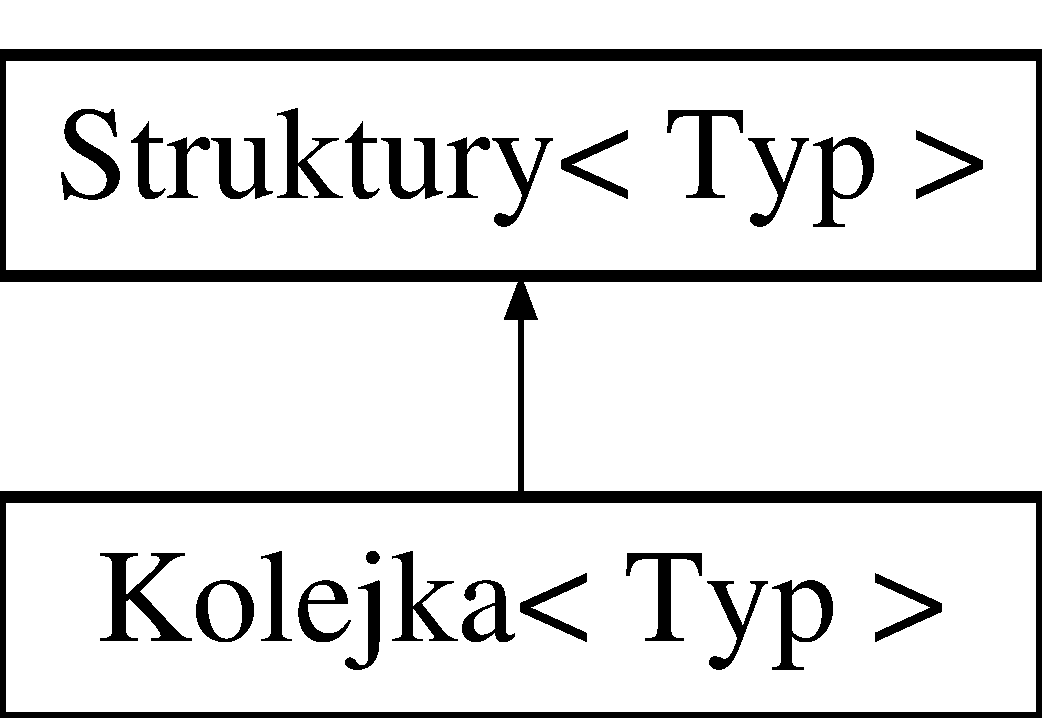
\includegraphics[height=2.000000cm]{class_kolejka}
\end{center}
\end{figure}
\subsection*{Classes}
\begin{DoxyCompactItemize}
\item 
struct \hyperlink{struct_kolejka_1_1_wezel}{Wezel}
\end{DoxyCompactItemize}
\subsection*{Public Member Functions}
\begin{DoxyCompactItemize}
\item 
\hyperlink{class_kolejka_a832240e4b63012eaa75f915986fdbb40}{Kolejka} ()
\begin{DoxyCompactList}\small\item\em Konstruktor. \end{DoxyCompactList}\item 
\hyperlink{class_kolejka_a4fe07cc3d71f815492010dc9bb665c7a}{$\sim$\-Kolejka} ()
\begin{DoxyCompactList}\small\item\em Destruktor. \end{DoxyCompactList}\item 
void \hyperlink{class_kolejka_a47121a1d8dd1b45bcf5411ab2d5bc099}{\-\_\-\-Pokaz} () const 
\begin{DoxyCompactList}\small\item\em Metoda wyswietlajaca elementu Kolejki. \end{DoxyCompactList}\item 
void \hyperlink{class_kolejka_a215bd2ca4b5db7ec861dfc78ee072858}{\-\_\-\-Push} (Typ k, unsigned int Pozycja=0)
\begin{DoxyCompactList}\small\item\em Metoda dodajaca nowy \hyperlink{struct_kolejka_1_1_wezel}{Wezel}. \end{DoxyCompactList}\item 
Typ \hyperlink{class_kolejka_ab26939041331d337b398819e3cc4443f}{\-\_\-\-Pop} (unsigned int Pozycja=0)
\begin{DoxyCompactList}\small\item\em Metda usuwajaca wezel. \end{DoxyCompactList}\item 
unsigned int \hyperlink{class_kolejka_ae76fad7ebe4fbc2bb7900e129a3677bc}{\-\_\-\-Rozmiar} () const 
\begin{DoxyCompactList}\small\item\em Metoda informujaca o obecnej ilosci Wezlow. \end{DoxyCompactList}\item 
bool \hyperlink{class_kolejka_aaeff23686afd067382547a9b37cb0187}{Czy\-Pusta} ()
\end{DoxyCompactItemize}
\subsection*{Private Member Functions}
\begin{DoxyCompactItemize}
\item 
void \hyperlink{class_kolejka_a607af93211b5e5e31123c633e1f1fcf2}{\-\_\-\-Zwolnij} ()
\begin{DoxyCompactList}\small\item\em Metoda zwalniajaca pamiec zajeta przez struktre. \end{DoxyCompactList}\end{DoxyCompactItemize}
\subsection*{Private Attributes}
\begin{DoxyCompactItemize}
\item 
\hyperlink{struct_kolejka_1_1_wezel}{Wezel} $\ast$ \hyperlink{class_kolejka_ad033655c575e128005d38099c10cfe89}{\-\_\-\-Pierwszy}
\begin{DoxyCompactList}\small\item\em Pole klasy \hyperlink{class_kolejka}{Kolejka}. \end{DoxyCompactList}\item 
\hyperlink{struct_kolejka_1_1_wezel}{Wezel} $\ast$ \hyperlink{class_kolejka_a0a7afd58e759661de14dbf9bab1a9d03}{\-\_\-\-Ostatni}
\begin{DoxyCompactList}\small\item\em Pole klasy \hyperlink{class_kolejka}{Kolejka}. \end{DoxyCompactList}\item 
unsigned int \hyperlink{class_kolejka_a803854da70e64a643364cac86c173dd6}{\-\_\-\-Ilosc}
\begin{DoxyCompactList}\small\item\em Pole klasy \hyperlink{class_kolejka}{Kolejka}. \end{DoxyCompactList}\end{DoxyCompactItemize}


\subsection{Detailed Description}
\subsubsection*{template$<$class Typ$>$class Kolejka$<$ Typ $>$}

Modeluje pojecie Kolejki. 

Klasa modeluje pojecie kolejki, dodajac nowy element na jej koniec i sciagajac pierwszy doddany element 

\subsection{Constructor \& Destructor Documentation}
\hypertarget{class_kolejka_a832240e4b63012eaa75f915986fdbb40}{\index{Kolejka@{Kolejka}!Kolejka@{Kolejka}}
\index{Kolejka@{Kolejka}!Kolejka@{Kolejka}}
\subsubsection[{Kolejka}]{\setlength{\rightskip}{0pt plus 5cm}template$<$class Typ $>$ {\bf Kolejka}$<$ Typ $>$\-::{\bf Kolejka} (
\begin{DoxyParamCaption}
{}
\end{DoxyParamCaption}
)\hspace{0.3cm}{\ttfamily [inline]}}}\label{class_kolejka_a832240e4b63012eaa75f915986fdbb40}


Konstruktor. 

Ustawia wskazniki na N\-U\-L\-L oraz zeruje ilosc elementow przy tworzeniu obiektow danej klasy \hypertarget{class_kolejka_a4fe07cc3d71f815492010dc9bb665c7a}{\index{Kolejka@{Kolejka}!$\sim$\-Kolejka@{$\sim$\-Kolejka}}
\index{$\sim$\-Kolejka@{$\sim$\-Kolejka}!Kolejka@{Kolejka}}
\subsubsection[{$\sim$\-Kolejka}]{\setlength{\rightskip}{0pt plus 5cm}template$<$class Typ $>$ {\bf Kolejka}$<$ Typ $>$\-::$\sim${\bf Kolejka} (
\begin{DoxyParamCaption}
{}
\end{DoxyParamCaption}
)\hspace{0.3cm}{\ttfamily [inline]}}}\label{class_kolejka_a4fe07cc3d71f815492010dc9bb665c7a}


Destruktor. 



\subsection{Member Function Documentation}
\hypertarget{class_kolejka_a47121a1d8dd1b45bcf5411ab2d5bc099}{\index{Kolejka@{Kolejka}!\-\_\-\-Pokaz@{\-\_\-\-Pokaz}}
\index{\-\_\-\-Pokaz@{\-\_\-\-Pokaz}!Kolejka@{Kolejka}}
\subsubsection[{\-\_\-\-Pokaz}]{\setlength{\rightskip}{0pt plus 5cm}template$<$class Typ $>$ void {\bf Kolejka}$<$ Typ $>$\-::\-\_\-\-Pokaz (
\begin{DoxyParamCaption}
{}
\end{DoxyParamCaption}
) const\hspace{0.3cm}{\ttfamily [inline]}, {\ttfamily [virtual]}}}\label{class_kolejka_a47121a1d8dd1b45bcf5411ab2d5bc099}


Metoda wyswietlajaca elementu Kolejki. 

Metoda ma za zadanie wyswietlic wszsytkie warotsci znajdujace sie w kolejce 

Implements \hyperlink{class_struktury_a9a4290d332a6a613f92d4d4bfe2577ae}{Struktury$<$ Typ $>$}.

\hypertarget{class_kolejka_ab26939041331d337b398819e3cc4443f}{\index{Kolejka@{Kolejka}!\-\_\-\-Pop@{\-\_\-\-Pop}}
\index{\-\_\-\-Pop@{\-\_\-\-Pop}!Kolejka@{Kolejka}}
\subsubsection[{\-\_\-\-Pop}]{\setlength{\rightskip}{0pt plus 5cm}template$<$class Typ $>$ Typ {\bf Kolejka}$<$ Typ $>$\-::\-\_\-\-Pop (
\begin{DoxyParamCaption}
\item[{unsigned int}]{Pozycja = {\ttfamily 0}}
\end{DoxyParamCaption}
)\hspace{0.3cm}{\ttfamily [inline]}, {\ttfamily [virtual]}}}\label{class_kolejka_ab26939041331d337b398819e3cc4443f}


Metda usuwajaca wezel. 

Metoda ma za zadanie usunac pierwszy dodany element z kolejki oraz ustawic wskaznik przed ostatniego elementu na N\-U\-L\-L 

Implements \hyperlink{class_struktury_a536345360bdb841d5462b578fe758b73}{Struktury$<$ Typ $>$}.

\hypertarget{class_kolejka_a215bd2ca4b5db7ec861dfc78ee072858}{\index{Kolejka@{Kolejka}!\-\_\-\-Push@{\-\_\-\-Push}}
\index{\-\_\-\-Push@{\-\_\-\-Push}!Kolejka@{Kolejka}}
\subsubsection[{\-\_\-\-Push}]{\setlength{\rightskip}{0pt plus 5cm}template$<$class Typ $>$ void {\bf Kolejka}$<$ Typ $>$\-::\-\_\-\-Push (
\begin{DoxyParamCaption}
\item[{Typ}]{k, }
\item[{unsigned int}]{Pozycja = {\ttfamily 0}}
\end{DoxyParamCaption}
)\hspace{0.3cm}{\ttfamily [inline]}, {\ttfamily [virtual]}}}\label{class_kolejka_a215bd2ca4b5db7ec861dfc78ee072858}


Metoda dodajaca nowy \hyperlink{struct_kolejka_1_1_wezel}{Wezel}. 

Metoda ma za zadanie dodac nowy wezel na koniec kolejki, umiescic w nim warosc zadana jako argument oraz pokazac wskaznkiem na ostatni \hyperlink{struct_kolejka_1_1_wezel}{Wezel} przed dodaniem nowego Wezla 
\begin{DoxyParams}[1]{Parameters}
\mbox{\tt in}  & {\em k} & -\/ Wartosc ktora zostanie umieszczona w odpowiednim polu Wezla \\
\hline
\end{DoxyParams}


Implements \hyperlink{class_struktury_aac09c019a75dd7bfda2f313733300c4c}{Struktury$<$ Typ $>$}.

\hypertarget{class_kolejka_ae76fad7ebe4fbc2bb7900e129a3677bc}{\index{Kolejka@{Kolejka}!\-\_\-\-Rozmiar@{\-\_\-\-Rozmiar}}
\index{\-\_\-\-Rozmiar@{\-\_\-\-Rozmiar}!Kolejka@{Kolejka}}
\subsubsection[{\-\_\-\-Rozmiar}]{\setlength{\rightskip}{0pt plus 5cm}template$<$class Typ $>$ unsigned int {\bf Kolejka}$<$ Typ $>$\-::\-\_\-\-Rozmiar (
\begin{DoxyParamCaption}
{}
\end{DoxyParamCaption}
) const\hspace{0.3cm}{\ttfamily [inline]}, {\ttfamily [virtual]}}}\label{class_kolejka_ae76fad7ebe4fbc2bb7900e129a3677bc}


Metoda informujaca o obecnej ilosci Wezlow. 

Metoda zwraca informacje o ilosci obecnie znajdujacych sie elementow w kolejce \begin{DoxyReturn}{Returns}
-\/ Zwraca ilosc elementow w kolejce 
\end{DoxyReturn}


Implements \hyperlink{class_struktury_a3ed3c70e26cefc242633abc13097acce}{Struktury$<$ Typ $>$}.

\hypertarget{class_kolejka_a607af93211b5e5e31123c633e1f1fcf2}{\index{Kolejka@{Kolejka}!\-\_\-\-Zwolnij@{\-\_\-\-Zwolnij}}
\index{\-\_\-\-Zwolnij@{\-\_\-\-Zwolnij}!Kolejka@{Kolejka}}
\subsubsection[{\-\_\-\-Zwolnij}]{\setlength{\rightskip}{0pt plus 5cm}template$<$class Typ $>$ void {\bf Kolejka}$<$ Typ $>$\-::\-\_\-\-Zwolnij (
\begin{DoxyParamCaption}
{}
\end{DoxyParamCaption}
)\hspace{0.3cm}{\ttfamily [inline]}, {\ttfamily [private]}, {\ttfamily [virtual]}}}\label{class_kolejka_a607af93211b5e5e31123c633e1f1fcf2}


Metoda zwalniajaca pamiec zajeta przez struktre. 

Metoda ma za zadanie zwolnij pamiec zajeta przez zaladowane do struktury dane, elementy sa usuwany dopoki wskaznik pokazujacy na poczatek kolejki nie bedzie wskazywal na N\-U\-L\-L 

Implements \hyperlink{class_struktury_aa85ab98de0f8bb1c257e6d1723d107f5}{Struktury$<$ Typ $>$}.

\hypertarget{class_kolejka_aaeff23686afd067382547a9b37cb0187}{\index{Kolejka@{Kolejka}!Czy\-Pusta@{Czy\-Pusta}}
\index{Czy\-Pusta@{Czy\-Pusta}!Kolejka@{Kolejka}}
\subsubsection[{Czy\-Pusta}]{\setlength{\rightskip}{0pt plus 5cm}template$<$class Typ $>$ bool {\bf Kolejka}$<$ Typ $>$\-::Czy\-Pusta (
\begin{DoxyParamCaption}
{}
\end{DoxyParamCaption}
)\hspace{0.3cm}{\ttfamily [inline]}}}\label{class_kolejka_aaeff23686afd067382547a9b37cb0187}


\subsection{Member Data Documentation}
\hypertarget{class_kolejka_a803854da70e64a643364cac86c173dd6}{\index{Kolejka@{Kolejka}!\-\_\-\-Ilosc@{\-\_\-\-Ilosc}}
\index{\-\_\-\-Ilosc@{\-\_\-\-Ilosc}!Kolejka@{Kolejka}}
\subsubsection[{\-\_\-\-Ilosc}]{\setlength{\rightskip}{0pt plus 5cm}template$<$class Typ $>$ unsigned int {\bf Kolejka}$<$ Typ $>$\-::\-\_\-\-Ilosc\hspace{0.3cm}{\ttfamily [private]}}}\label{class_kolejka_a803854da70e64a643364cac86c173dd6}


Pole klasy \hyperlink{class_kolejka}{Kolejka}. 

Pole przechowuje inrofmracje o ilosci obecnie znajdujacych sie elementow w kolejce \hypertarget{class_kolejka_a0a7afd58e759661de14dbf9bab1a9d03}{\index{Kolejka@{Kolejka}!\-\_\-\-Ostatni@{\-\_\-\-Ostatni}}
\index{\-\_\-\-Ostatni@{\-\_\-\-Ostatni}!Kolejka@{Kolejka}}
\subsubsection[{\-\_\-\-Ostatni}]{\setlength{\rightskip}{0pt plus 5cm}template$<$class Typ $>$ {\bf Wezel}$\ast$ {\bf Kolejka}$<$ Typ $>$\-::\-\_\-\-Ostatni\hspace{0.3cm}{\ttfamily [private]}}}\label{class_kolejka_a0a7afd58e759661de14dbf9bab1a9d03}


Pole klasy \hyperlink{class_kolejka}{Kolejka}. 

Pole jest wskaznikiem na ostatni element kolejki \hypertarget{class_kolejka_ad033655c575e128005d38099c10cfe89}{\index{Kolejka@{Kolejka}!\-\_\-\-Pierwszy@{\-\_\-\-Pierwszy}}
\index{\-\_\-\-Pierwszy@{\-\_\-\-Pierwszy}!Kolejka@{Kolejka}}
\subsubsection[{\-\_\-\-Pierwszy}]{\setlength{\rightskip}{0pt plus 5cm}template$<$class Typ $>$ {\bf Wezel}$\ast$ {\bf Kolejka}$<$ Typ $>$\-::\-\_\-\-Pierwszy\hspace{0.3cm}{\ttfamily [private]}}}\label{class_kolejka_ad033655c575e128005d38099c10cfe89}


Pole klasy \hyperlink{class_kolejka}{Kolejka}. 

Pole jest wskaznikiem na pierwszy element kolejki 

The documentation for this class was generated from the following file\-:\begin{DoxyCompactItemize}
\item 
/home/bartolomeo/209255/prj/inc/\hyperlink{_kolejka_8hh}{Kolejka.\-hh}\end{DoxyCompactItemize}

\hypertarget{class_lista}{\section{Lista$<$ Typ $>$ Class Template Reference}
\label{class_lista}\index{Lista$<$ Typ $>$@{Lista$<$ Typ $>$}}
}


{\ttfamily \#include $<$Lista.\-hh$>$}

Inheritance diagram for Lista$<$ Typ $>$\-:\begin{figure}[H]
\begin{center}
\leavevmode
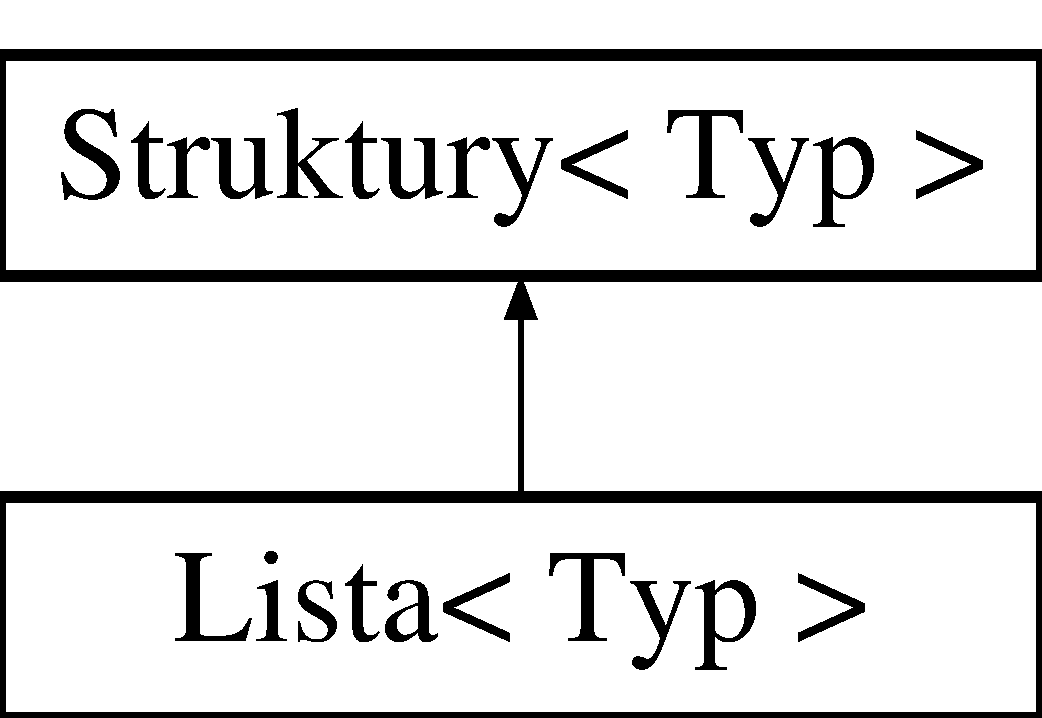
\includegraphics[height=2.000000cm]{class_lista}
\end{center}
\end{figure}
\subsection*{Classes}
\begin{DoxyCompactItemize}
\item 
struct \hyperlink{struct_lista_1_1_wezel}{Wezel}
\end{DoxyCompactItemize}
\subsection*{Public Member Functions}
\begin{DoxyCompactItemize}
\item 
void \hyperlink{class_lista_a5969ea939160694d8eea3cff3ac34cb8}{\-\_\-\-Push} (Typ Wart, unsigned int Poz)
\begin{DoxyCompactList}\small\item\em Metoda dodajaca \hyperlink{struct_lista_1_1_wezel}{Wezel}. \end{DoxyCompactList}\item 
Typ \hyperlink{class_lista_a515f4dd7a4ffdfb2fdc12a5fa28e97a4}{\-\_\-\-Pop} (unsigned int Pozycja)
\begin{DoxyCompactList}\small\item\em Metoda usuwajaca \hyperlink{struct_lista_1_1_wezel}{Wezel}. \end{DoxyCompactList}\item 
unsigned int \hyperlink{class_lista_a4fb94c2a9d576a4a32acd1e63f339d38}{\-\_\-\-Rozmiar} () const 
\begin{DoxyCompactList}\small\item\em Metoda informujaca o ilosci wezlow. \end{DoxyCompactList}\item 
\hyperlink{class_lista_a674e0e60c11e301bcfb39ca4a9102f9a}{Lista} ()
\begin{DoxyCompactList}\small\item\em Konstruktor. \end{DoxyCompactList}\item 
\hyperlink{class_lista_acfd996dad8df54ffaa389fdcbe04f643}{$\sim$\-Lista} ()
\begin{DoxyCompactList}\small\item\em Destruktor Usuwa wskaznik. \end{DoxyCompactList}\item 
void \hyperlink{class_lista_abae4fe58b5a4225b0df8d98caa65db75}{\-\_\-\-Pokaz} () const 
\begin{DoxyCompactList}\small\item\em Konstruktor Kopiujacy. \end{DoxyCompactList}\end{DoxyCompactItemize}
\subsection*{Private Member Functions}
\begin{DoxyCompactItemize}
\item 
void \hyperlink{class_lista_a3ff3e2f58bd3b1d1b11f9ad68948a321}{\-\_\-\-Zwolnij} ()
\begin{DoxyCompactList}\small\item\em Metoda zwalniajaca pamiec zajeta przez struktre. \end{DoxyCompactList}\end{DoxyCompactItemize}
\subsection*{Private Attributes}
\begin{DoxyCompactItemize}
\item 
\hyperlink{struct_lista_1_1_wezel}{Wezel} $\ast$ \hyperlink{class_lista_a771f55b84b2b9b3bee3fd68db71e273a}{Glowa}
\begin{DoxyCompactList}\small\item\em Pole klasy \hyperlink{class_lista}{Lista} Wskaznik na nowo dodany \hyperlink{struct_lista_1_1_wezel}{Wezel}. \end{DoxyCompactList}\item 
unsigned int \hyperlink{class_lista_a8b2341ebf8c4591c96650e68c1b7548b}{\-\_\-\-Ilosc}
\begin{DoxyCompactList}\small\item\em Pole klasy \hyperlink{class_lista}{Lista} Pole przechowuje bierzaca ilosc elementow listy. \end{DoxyCompactList}\end{DoxyCompactItemize}


\subsection{Constructor \& Destructor Documentation}
\hypertarget{class_lista_a674e0e60c11e301bcfb39ca4a9102f9a}{\index{Lista@{Lista}!Lista@{Lista}}
\index{Lista@{Lista}!Lista@{Lista}}
\subsubsection[{Lista}]{\setlength{\rightskip}{0pt plus 5cm}template$<$class Typ $>$ {\bf Lista}$<$ Typ $>$\-::{\bf Lista} (
\begin{DoxyParamCaption}
{}
\end{DoxyParamCaption}
)\hspace{0.3cm}{\ttfamily [inline]}}}\label{class_lista_a674e0e60c11e301bcfb39ca4a9102f9a}


Konstruktor. 

Konstruktor ustawia wskaznik na N\-U\-L\-L i zeruje ilosc wezlow listy \hypertarget{class_lista_acfd996dad8df54ffaa389fdcbe04f643}{\index{Lista@{Lista}!$\sim$\-Lista@{$\sim$\-Lista}}
\index{$\sim$\-Lista@{$\sim$\-Lista}!Lista@{Lista}}
\subsubsection[{$\sim$\-Lista}]{\setlength{\rightskip}{0pt plus 5cm}template$<$class Typ $>$ {\bf Lista}$<$ Typ $>$\-::$\sim${\bf Lista} (
\begin{DoxyParamCaption}
{}
\end{DoxyParamCaption}
)\hspace{0.3cm}{\ttfamily [inline]}}}\label{class_lista_acfd996dad8df54ffaa389fdcbe04f643}


Destruktor Usuwa wskaznik. 



\subsection{Member Function Documentation}
\hypertarget{class_lista_abae4fe58b5a4225b0df8d98caa65db75}{\index{Lista@{Lista}!\-\_\-\-Pokaz@{\-\_\-\-Pokaz}}
\index{\-\_\-\-Pokaz@{\-\_\-\-Pokaz}!Lista@{Lista}}
\subsubsection[{\-\_\-\-Pokaz}]{\setlength{\rightskip}{0pt plus 5cm}template$<$class Typ $>$ void {\bf Lista}$<$ Typ $>$\-::\-\_\-\-Pokaz (
\begin{DoxyParamCaption}
{}
\end{DoxyParamCaption}
) const\hspace{0.3cm}{\ttfamily [inline]}, {\ttfamily [virtual]}}}\label{class_lista_abae4fe58b5a4225b0df8d98caa65db75}


Konstruktor Kopiujacy. 

Metoda wyswietlajaca elementy Listy

Metoda ma za zadanie wyswietlic wszsytkie warotsci znajdujace sie na Liscie 

Implements \hyperlink{class_struktury_a9a4290d332a6a613f92d4d4bfe2577ae}{Struktury$<$ Typ $>$}.

\hypertarget{class_lista_a515f4dd7a4ffdfb2fdc12a5fa28e97a4}{\index{Lista@{Lista}!\-\_\-\-Pop@{\-\_\-\-Pop}}
\index{\-\_\-\-Pop@{\-\_\-\-Pop}!Lista@{Lista}}
\subsubsection[{\-\_\-\-Pop}]{\setlength{\rightskip}{0pt plus 5cm}template$<$class Typ $>$ Typ {\bf Lista}$<$ Typ $>$\-::\-\_\-\-Pop (
\begin{DoxyParamCaption}
\item[{unsigned int}]{Pozycja}
\end{DoxyParamCaption}
)\hspace{0.3cm}{\ttfamily [inline]}, {\ttfamily [virtual]}}}\label{class_lista_a515f4dd7a4ffdfb2fdc12a5fa28e97a4}


Metoda usuwajaca \hyperlink{struct_lista_1_1_wezel}{Wezel}. 

Metoda ma za zadanie usunac wezel zgodny z argumentem metody \hyperlink{struct_lista_1_1_wezel}{Wezel} zosatnie usuniety, a sasiednie elementy zostana polaczaone wskazniekiem


\begin{DoxyParams}[1]{Parameters}
\mbox{\tt in}  & {\em Pozycja} & -\/ Numer Wezla ktory zostanie usuniety \\
\hline
\end{DoxyParams}


Implements \hyperlink{class_struktury_a536345360bdb841d5462b578fe758b73}{Struktury$<$ Typ $>$}.

\hypertarget{class_lista_a5969ea939160694d8eea3cff3ac34cb8}{\index{Lista@{Lista}!\-\_\-\-Push@{\-\_\-\-Push}}
\index{\-\_\-\-Push@{\-\_\-\-Push}!Lista@{Lista}}
\subsubsection[{\-\_\-\-Push}]{\setlength{\rightskip}{0pt plus 5cm}template$<$class Typ $>$ void {\bf Lista}$<$ Typ $>$\-::\-\_\-\-Push (
\begin{DoxyParamCaption}
\item[{Typ}]{Wart, }
\item[{unsigned int}]{Poz}
\end{DoxyParamCaption}
)\hspace{0.3cm}{\ttfamily [inline]}, {\ttfamily [virtual]}}}\label{class_lista_a5969ea939160694d8eea3cff3ac34cb8}


Metoda dodajaca \hyperlink{struct_lista_1_1_wezel}{Wezel}. 

Metoda ma za zadanie dodac element do listy w zaleznosci od argumentu miejscu i usatwic wartosc zadana przez argument 
\begin{DoxyParams}[1]{Parameters}
\mbox{\tt in}  & {\em wart} & -\/ Wartosc jaka zostana dodana do Wezla \\
\hline
\mbox{\tt in}  & {\em poz} & -\/ Pozycja w ktorej zosatnie dodany \hyperlink{struct_lista_1_1_wezel}{Wezel} \\
\hline
\end{DoxyParams}


Implements \hyperlink{class_struktury_aac09c019a75dd7bfda2f313733300c4c}{Struktury$<$ Typ $>$}.

\hypertarget{class_lista_a4fb94c2a9d576a4a32acd1e63f339d38}{\index{Lista@{Lista}!\-\_\-\-Rozmiar@{\-\_\-\-Rozmiar}}
\index{\-\_\-\-Rozmiar@{\-\_\-\-Rozmiar}!Lista@{Lista}}
\subsubsection[{\-\_\-\-Rozmiar}]{\setlength{\rightskip}{0pt plus 5cm}template$<$class Typ $>$ unsigned int {\bf Lista}$<$ Typ $>$\-::\-\_\-\-Rozmiar (
\begin{DoxyParamCaption}
{}
\end{DoxyParamCaption}
) const\hspace{0.3cm}{\ttfamily [inline]}, {\ttfamily [virtual]}}}\label{class_lista_a4fb94c2a9d576a4a32acd1e63f339d38}


Metoda informujaca o ilosci wezlow. 

Metoda zwraca informajce o ilosci aktualnych wezlow listy \begin{DoxyReturn}{Returns}
-\/ Ilosc elementow listy 
\end{DoxyReturn}


Implements \hyperlink{class_struktury_a3ed3c70e26cefc242633abc13097acce}{Struktury$<$ Typ $>$}.

\hypertarget{class_lista_a3ff3e2f58bd3b1d1b11f9ad68948a321}{\index{Lista@{Lista}!\-\_\-\-Zwolnij@{\-\_\-\-Zwolnij}}
\index{\-\_\-\-Zwolnij@{\-\_\-\-Zwolnij}!Lista@{Lista}}
\subsubsection[{\-\_\-\-Zwolnij}]{\setlength{\rightskip}{0pt plus 5cm}template$<$class Typ $>$ void {\bf Lista}$<$ Typ $>$\-::\-\_\-\-Zwolnij (
\begin{DoxyParamCaption}
{}
\end{DoxyParamCaption}
)\hspace{0.3cm}{\ttfamily [inline]}, {\ttfamily [private]}, {\ttfamily [virtual]}}}\label{class_lista_a3ff3e2f58bd3b1d1b11f9ad68948a321}


Metoda zwalniajaca pamiec zajeta przez struktre. 

Metoda ma za zadanie zwolnij pamiec zajeta przez zaladowane do struktury dane, elementy sa usuwany dopoki wskaznik pokazujacy na poczatek listy nie bedzie wskazywal na N\-U\-L\-L 

Implements \hyperlink{class_struktury_aa85ab98de0f8bb1c257e6d1723d107f5}{Struktury$<$ Typ $>$}.



\subsection{Member Data Documentation}
\hypertarget{class_lista_a8b2341ebf8c4591c96650e68c1b7548b}{\index{Lista@{Lista}!\-\_\-\-Ilosc@{\-\_\-\-Ilosc}}
\index{\-\_\-\-Ilosc@{\-\_\-\-Ilosc}!Lista@{Lista}}
\subsubsection[{\-\_\-\-Ilosc}]{\setlength{\rightskip}{0pt plus 5cm}template$<$class Typ $>$ unsigned int {\bf Lista}$<$ Typ $>$\-::\-\_\-\-Ilosc\hspace{0.3cm}{\ttfamily [private]}}}\label{class_lista_a8b2341ebf8c4591c96650e68c1b7548b}


Pole klasy \hyperlink{class_lista}{Lista} Pole przechowuje bierzaca ilosc elementow listy. 

\hypertarget{class_lista_a771f55b84b2b9b3bee3fd68db71e273a}{\index{Lista@{Lista}!Glowa@{Glowa}}
\index{Glowa@{Glowa}!Lista@{Lista}}
\subsubsection[{Glowa}]{\setlength{\rightskip}{0pt plus 5cm}template$<$class Typ $>$ {\bf Wezel}$\ast$ {\bf Lista}$<$ Typ $>$\-::Glowa\hspace{0.3cm}{\ttfamily [private]}}}\label{class_lista_a771f55b84b2b9b3bee3fd68db71e273a}


Pole klasy \hyperlink{class_lista}{Lista} Wskaznik na nowo dodany \hyperlink{struct_lista_1_1_wezel}{Wezel}. 



The documentation for this class was generated from the following file\-:\begin{DoxyCompactItemize}
\item 
/home/bartolomeo/209255/prj/inc/\hyperlink{_lista_8hh}{Lista.\-hh}\end{DoxyCompactItemize}

\hypertarget{class_stos_tab}{\section{Stos\-Tab$<$ Typ $>$ Class Template Reference}
\label{class_stos_tab}\index{Stos\-Tab$<$ Typ $>$@{Stos\-Tab$<$ Typ $>$}}
}


{\ttfamily \#include $<$Stos\-Tab.\-hh$>$}

Inheritance diagram for Stos\-Tab$<$ Typ $>$\-:\begin{figure}[H]
\begin{center}
\leavevmode
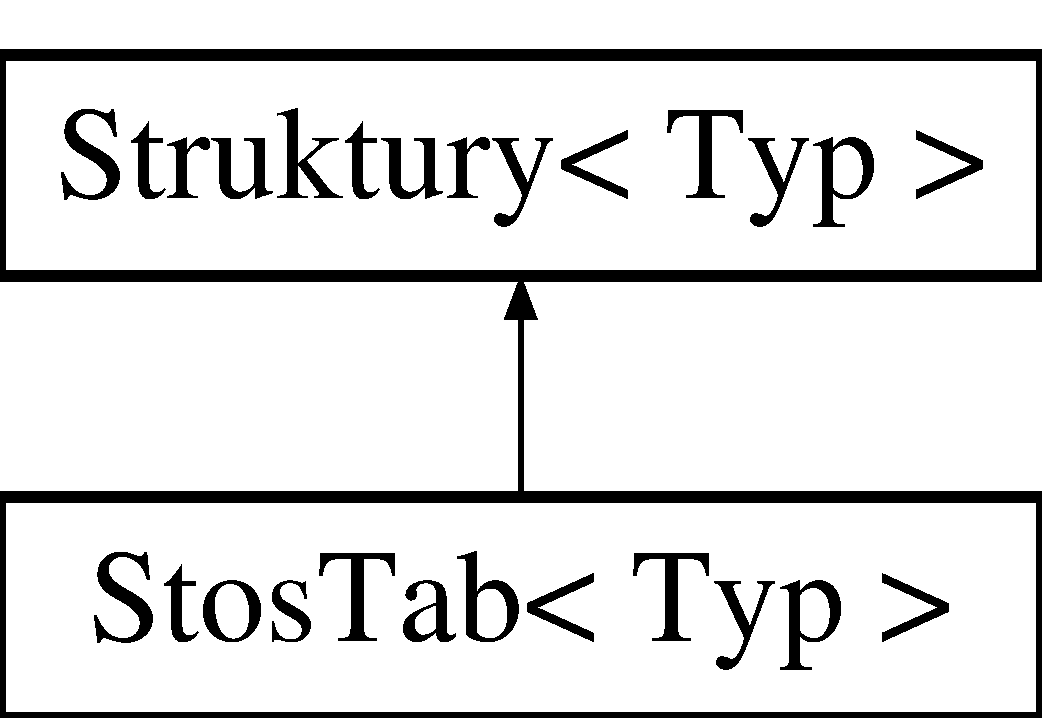
\includegraphics[height=2.000000cm]{class_stos_tab}
\end{center}
\end{figure}
\subsection*{Public Member Functions}
\begin{DoxyCompactItemize}
\item 
void \hyperlink{class_stos_tab_aec0cb259c6f044fa7d3b367dc1baca5c}{\-\_\-\-Zwolnij} ()
\item 
\hyperlink{class_stos_tab_a347bc350ea6ff8ad86b853895db5e7a9}{Stos\-Tab} ()
\begin{DoxyCompactList}\small\item\em Konstruktor Podczas tworzenia obiektu tej klasy automatycznie alokowana jest tablica o rozmiarze 1 oraz ustawienie obecnej liczby elementow listy na 0. \end{DoxyCompactList}\item 
\hyperlink{class_stos_tab_a5972345c1b71597d11330f8953dec03d}{Stos\-Tab} (const \hyperlink{class_stos_tab}{Stos\-Tab} \&K)
\begin{DoxyCompactList}\small\item\em Konstruktor Kopiujacy. \end{DoxyCompactList}\item 
virtual \hyperlink{class_stos_tab_a580b0a918a829377698f475a5f75457b}{$\sim$\-Stos\-Tab} ()
\begin{DoxyCompactList}\small\item\em Destruktor obiektu. \end{DoxyCompactList}\item 
void \hyperlink{class_stos_tab_a1b3c30902f28bf819ea5864c85ebede9}{\-\_\-\-Pokaz} () const 
\begin{DoxyCompactList}\small\item\em Metoda wypisujaca elemeny Stosu. \end{DoxyCompactList}\item 
Typ \hyperlink{class_stos_tab_a43e5e031570e69dc27fc11feca969645}{\-\_\-\-Pop} (unsigned int Pozycja=0)
\begin{DoxyCompactList}\small\item\em Metoda sciagajaca element ze stosu. \end{DoxyCompactList}\item 
void \hyperlink{class_stos_tab_a73c95fc8151510c21c5567e85296ea31}{\-\_\-\-Push} (Typ k, unsigned int Pozycja=0)
\begin{DoxyCompactList}\small\item\em Metoda dodajaca elemet do tablicy. \end{DoxyCompactList}\item 
unsigned int \hyperlink{class_stos_tab_a51b2da61d6c4c2085646b84395c2d3c0}{\-\_\-\-Rozmiar} () const 
\begin{DoxyCompactList}\small\item\em Metoda zwracajaca rozmiar listy. \end{DoxyCompactList}\item 
bool \hyperlink{class_stos_tab_af75e71d75e10fcce0b2751c84728b38c}{Czy\-Pusty} ()
\end{DoxyCompactItemize}
\subsection*{Private Attributes}
\begin{DoxyCompactItemize}
\item 
Typ $\ast$ \hyperlink{class_stos_tab_ab6a9150fc50f2eb508a6c8026816631b}{\-\_\-\-L}
\begin{DoxyCompactList}\small\item\em Pole klasy \hyperlink{class_stos_tab}{Stos\-Tab}. \end{DoxyCompactList}\item 
unsigned int \hyperlink{class_stos_tab_abb7d52d46fdaf90dc2f3acb421bf7af6}{\-\_\-\-Rozmiar\-L}
\begin{DoxyCompactList}\small\item\em Pole Klasy \hyperlink{class_stos_tab}{Stos\-Tab}. \end{DoxyCompactList}\item 
unsigned int \hyperlink{class_stos_tab_a4db33c7f5b5f57b4d755a1beb59852dc}{\-\_\-\-Rozmiar\-T}
\begin{DoxyCompactList}\small\item\em Pole Klasy \hyperlink{class_stos_tab}{Stos\-Tab}. \end{DoxyCompactList}\end{DoxyCompactItemize}


\subsection{Constructor \& Destructor Documentation}
\hypertarget{class_stos_tab_a347bc350ea6ff8ad86b853895db5e7a9}{\index{Stos\-Tab@{Stos\-Tab}!Stos\-Tab@{Stos\-Tab}}
\index{Stos\-Tab@{Stos\-Tab}!StosTab@{Stos\-Tab}}
\subsubsection[{Stos\-Tab}]{\setlength{\rightskip}{0pt plus 5cm}template$<$class Typ $>$ {\bf Stos\-Tab}$<$ Typ $>$\-::{\bf Stos\-Tab} (
\begin{DoxyParamCaption}
{}
\end{DoxyParamCaption}
)\hspace{0.3cm}{\ttfamily [inline]}}}\label{class_stos_tab_a347bc350ea6ff8ad86b853895db5e7a9}


Konstruktor Podczas tworzenia obiektu tej klasy automatycznie alokowana jest tablica o rozmiarze 1 oraz ustawienie obecnej liczby elementow listy na 0. 

\hypertarget{class_stos_tab_a5972345c1b71597d11330f8953dec03d}{\index{Stos\-Tab@{Stos\-Tab}!Stos\-Tab@{Stos\-Tab}}
\index{Stos\-Tab@{Stos\-Tab}!StosTab@{Stos\-Tab}}
\subsubsection[{Stos\-Tab}]{\setlength{\rightskip}{0pt plus 5cm}template$<$class Typ $>$ {\bf Stos\-Tab}$<$ Typ $>$\-::{\bf Stos\-Tab} (
\begin{DoxyParamCaption}
\item[{const {\bf Stos\-Tab}$<$ Typ $>$ \&}]{K}
\end{DoxyParamCaption}
)\hspace{0.3cm}{\ttfamily [inline]}}}\label{class_stos_tab_a5972345c1b71597d11330f8953dec03d}


Konstruktor Kopiujacy. 

\hypertarget{class_stos_tab_a580b0a918a829377698f475a5f75457b}{\index{Stos\-Tab@{Stos\-Tab}!$\sim$\-Stos\-Tab@{$\sim$\-Stos\-Tab}}
\index{$\sim$\-Stos\-Tab@{$\sim$\-Stos\-Tab}!StosTab@{Stos\-Tab}}
\subsubsection[{$\sim$\-Stos\-Tab}]{\setlength{\rightskip}{0pt plus 5cm}template$<$class Typ $>$ virtual {\bf Stos\-Tab}$<$ Typ $>$\-::$\sim${\bf Stos\-Tab} (
\begin{DoxyParamCaption}
{}
\end{DoxyParamCaption}
)\hspace{0.3cm}{\ttfamily [inline]}}}\label{class_stos_tab_a580b0a918a829377698f475a5f75457b}


Destruktor obiektu. 



\subsection{Member Function Documentation}
\hypertarget{class_stos_tab_a1b3c30902f28bf819ea5864c85ebede9}{\index{Stos\-Tab@{Stos\-Tab}!\-\_\-\-Pokaz@{\-\_\-\-Pokaz}}
\index{\-\_\-\-Pokaz@{\-\_\-\-Pokaz}!StosTab@{Stos\-Tab}}
\subsubsection[{\-\_\-\-Pokaz}]{\setlength{\rightskip}{0pt plus 5cm}template$<$class Typ $>$ void {\bf Stos\-Tab}$<$ Typ $>$\-::\-\_\-\-Pokaz (
\begin{DoxyParamCaption}
{}
\end{DoxyParamCaption}
) const\hspace{0.3cm}{\ttfamily [inline]}, {\ttfamily [virtual]}}}\label{class_stos_tab_a1b3c30902f28bf819ea5864c85ebede9}


Metoda wypisujaca elemeny Stosu. 

Metoda ma za zadanie wypisac wszystkie elementy znajdujace sie obecnie na liscie danych 

Implements \hyperlink{class_struktury_a9a4290d332a6a613f92d4d4bfe2577ae}{Struktury$<$ Typ $>$}.

\hypertarget{class_stos_tab_a43e5e031570e69dc27fc11feca969645}{\index{Stos\-Tab@{Stos\-Tab}!\-\_\-\-Pop@{\-\_\-\-Pop}}
\index{\-\_\-\-Pop@{\-\_\-\-Pop}!StosTab@{Stos\-Tab}}
\subsubsection[{\-\_\-\-Pop}]{\setlength{\rightskip}{0pt plus 5cm}template$<$class Typ $>$ Typ {\bf Stos\-Tab}$<$ Typ $>$\-::\-\_\-\-Pop (
\begin{DoxyParamCaption}
\item[{unsigned int}]{Pozycja = {\ttfamily 0}}
\end{DoxyParamCaption}
)\hspace{0.3cm}{\ttfamily [inline]}, {\ttfamily [virtual]}}}\label{class_stos_tab_a43e5e031570e69dc27fc11feca969645}


Metoda sciagajaca element ze stosu. 

Metoda ma za zadanie sciagnac ostatni element stosu, w przypadku gdy tablica jest do połowy pusta nastepuje utworzenie nowej tablicy o dwa razy mniejszym rozmiarze 
\begin{DoxyParams}[1]{Parameters}
\mbox{\tt in}  & {\em Pozycja} & -\/ numer elementy kotry zostanie usuniety z listy i zostanie zwrocona jego wartosc\\
\hline
\end{DoxyParams}
\begin{DoxyReturn}{Returns}
Zwraca wybrany przez uzytkownika element 
\end{DoxyReturn}


Implements \hyperlink{class_struktury_a536345360bdb841d5462b578fe758b73}{Struktury$<$ Typ $>$}.

\hypertarget{class_stos_tab_a73c95fc8151510c21c5567e85296ea31}{\index{Stos\-Tab@{Stos\-Tab}!\-\_\-\-Push@{\-\_\-\-Push}}
\index{\-\_\-\-Push@{\-\_\-\-Push}!StosTab@{Stos\-Tab}}
\subsubsection[{\-\_\-\-Push}]{\setlength{\rightskip}{0pt plus 5cm}template$<$class Typ $>$ void {\bf Stos\-Tab}$<$ Typ $>$\-::\-\_\-\-Push (
\begin{DoxyParamCaption}
\item[{Typ}]{k, }
\item[{unsigned int}]{Pozycja = {\ttfamily 0}}
\end{DoxyParamCaption}
)\hspace{0.3cm}{\ttfamily [inline]}, {\ttfamily [virtual]}}}\label{class_stos_tab_a73c95fc8151510c21c5567e85296ea31}


Metoda dodajaca elemet do tablicy. 

Metoda ma za zadanie dodac nowy element na koncu stosu, w przypadku zapelnienia tablicy nastepuje utworzenie nowej tablicy i przepisanie elementow


\begin{DoxyParams}[1]{Parameters}
\mbox{\tt in}  & {\em k} & -\/ wartosc jaka chcemy dodac do listy \\
\hline
\mbox{\tt in}  & {\em Pozycja} & -\/ Pozycja na ktorej chcemy dodac wartosc \\
\hline
\end{DoxyParams}


Implements \hyperlink{class_struktury_aac09c019a75dd7bfda2f313733300c4c}{Struktury$<$ Typ $>$}.

\hypertarget{class_stos_tab_a51b2da61d6c4c2085646b84395c2d3c0}{\index{Stos\-Tab@{Stos\-Tab}!\-\_\-\-Rozmiar@{\-\_\-\-Rozmiar}}
\index{\-\_\-\-Rozmiar@{\-\_\-\-Rozmiar}!StosTab@{Stos\-Tab}}
\subsubsection[{\-\_\-\-Rozmiar}]{\setlength{\rightskip}{0pt plus 5cm}template$<$class Typ $>$ unsigned int {\bf Stos\-Tab}$<$ Typ $>$\-::\-\_\-\-Rozmiar (
\begin{DoxyParamCaption}
{}
\end{DoxyParamCaption}
) const\hspace{0.3cm}{\ttfamily [inline]}, {\ttfamily [virtual]}}}\label{class_stos_tab_a51b2da61d6c4c2085646b84395c2d3c0}


Metoda zwracajaca rozmiar listy. 

Metoda zwraca informacje o obecnej ilosci danych w strukturze

\begin{DoxyReturn}{Returns}
Zwraca ilosc elementow listy 
\end{DoxyReturn}


Implements \hyperlink{class_struktury_a3ed3c70e26cefc242633abc13097acce}{Struktury$<$ Typ $>$}.

\hypertarget{class_stos_tab_aec0cb259c6f044fa7d3b367dc1baca5c}{\index{Stos\-Tab@{Stos\-Tab}!\-\_\-\-Zwolnij@{\-\_\-\-Zwolnij}}
\index{\-\_\-\-Zwolnij@{\-\_\-\-Zwolnij}!StosTab@{Stos\-Tab}}
\subsubsection[{\-\_\-\-Zwolnij}]{\setlength{\rightskip}{0pt plus 5cm}template$<$class Typ $>$ void {\bf Stos\-Tab}$<$ Typ $>$\-::\-\_\-\-Zwolnij (
\begin{DoxyParamCaption}
{}
\end{DoxyParamCaption}
)\hspace{0.3cm}{\ttfamily [inline]}, {\ttfamily [virtual]}}}\label{class_stos_tab_aec0cb259c6f044fa7d3b367dc1baca5c}
Metoda zwalniajaca pamiec

Metoda ma za zadanie zwolnij pamiec zajmowana przez dane, dopoki ilosc elementow listy nie wynosi 0 wykonywana jest metoda \-\_\-\-Pop, aby oproznic stos i zwolnic pamiec 

Implements \hyperlink{class_struktury_aa85ab98de0f8bb1c257e6d1723d107f5}{Struktury$<$ Typ $>$}.

\hypertarget{class_stos_tab_af75e71d75e10fcce0b2751c84728b38c}{\index{Stos\-Tab@{Stos\-Tab}!Czy\-Pusty@{Czy\-Pusty}}
\index{Czy\-Pusty@{Czy\-Pusty}!StosTab@{Stos\-Tab}}
\subsubsection[{Czy\-Pusty}]{\setlength{\rightskip}{0pt plus 5cm}template$<$class Typ $>$ bool {\bf Stos\-Tab}$<$ Typ $>$\-::Czy\-Pusty (
\begin{DoxyParamCaption}
{}
\end{DoxyParamCaption}
)\hspace{0.3cm}{\ttfamily [inline]}}}\label{class_stos_tab_af75e71d75e10fcce0b2751c84728b38c}


\subsection{Member Data Documentation}
\hypertarget{class_stos_tab_ab6a9150fc50f2eb508a6c8026816631b}{\index{Stos\-Tab@{Stos\-Tab}!\-\_\-\-L@{\-\_\-\-L}}
\index{\-\_\-\-L@{\-\_\-\-L}!StosTab@{Stos\-Tab}}
\subsubsection[{\-\_\-\-L}]{\setlength{\rightskip}{0pt plus 5cm}template$<$class Typ $>$ Typ$\ast$ {\bf Stos\-Tab}$<$ Typ $>$\-::\-\_\-\-L\hspace{0.3cm}{\ttfamily [private]}}}\label{class_stos_tab_ab6a9150fc50f2eb508a6c8026816631b}


Pole klasy \hyperlink{class_stos_tab}{Stos\-Tab}. 

Pole zawiera wskaznik na typ calkowity, sluzy do alokacji pamieci na dynamiczna tablice \hypertarget{class_stos_tab_abb7d52d46fdaf90dc2f3acb421bf7af6}{\index{Stos\-Tab@{Stos\-Tab}!\-\_\-\-Rozmiar\-L@{\-\_\-\-Rozmiar\-L}}
\index{\-\_\-\-Rozmiar\-L@{\-\_\-\-Rozmiar\-L}!StosTab@{Stos\-Tab}}
\subsubsection[{\-\_\-\-Rozmiar\-L}]{\setlength{\rightskip}{0pt plus 5cm}template$<$class Typ $>$ unsigned int {\bf Stos\-Tab}$<$ Typ $>$\-::\-\_\-\-Rozmiar\-L\hspace{0.3cm}{\ttfamily [private]}}}\label{class_stos_tab_abb7d52d46fdaf90dc2f3acb421bf7af6}


Pole Klasy \hyperlink{class_stos_tab}{Stos\-Tab}. 

Pole przechowuje informacje o ilosci obecnie znajdujacych sie elementow na liscie danych \hypertarget{class_stos_tab_a4db33c7f5b5f57b4d755a1beb59852dc}{\index{Stos\-Tab@{Stos\-Tab}!\-\_\-\-Rozmiar\-T@{\-\_\-\-Rozmiar\-T}}
\index{\-\_\-\-Rozmiar\-T@{\-\_\-\-Rozmiar\-T}!StosTab@{Stos\-Tab}}
\subsubsection[{\-\_\-\-Rozmiar\-T}]{\setlength{\rightskip}{0pt plus 5cm}template$<$class Typ $>$ unsigned int {\bf Stos\-Tab}$<$ Typ $>$\-::\-\_\-\-Rozmiar\-T\hspace{0.3cm}{\ttfamily [private]}}}\label{class_stos_tab_a4db33c7f5b5f57b4d755a1beb59852dc}


Pole Klasy \hyperlink{class_stos_tab}{Stos\-Tab}. 

Pole przechowuje informacje o obecnycm rozmiarze tablicy danych 

The documentation for this class was generated from the following file\-:\begin{DoxyCompactItemize}
\item 
/home/bartolomeo/209255/prj/inc/\hyperlink{_stos_tab_8hh}{Stos\-Tab.\-hh}\end{DoxyCompactItemize}

\hypertarget{class_struktury}{\section{Struktury$<$ Typ $>$ Class Template Reference}
\label{class_struktury}\index{Struktury$<$ Typ $>$@{Struktury$<$ Typ $>$}}
}


Modeluje pojecie \hyperlink{class_struktury}{Struktury} danych, klasa bazowa dla Stosu,Kolejki i Listy,zarowno w implemenetacji wskaznikowej jak i tablicowej.  




{\ttfamily \#include $<$Struktury.\-hh$>$}

Inheritance diagram for Struktury$<$ Typ $>$\-:\begin{figure}[H]
\begin{center}
\leavevmode
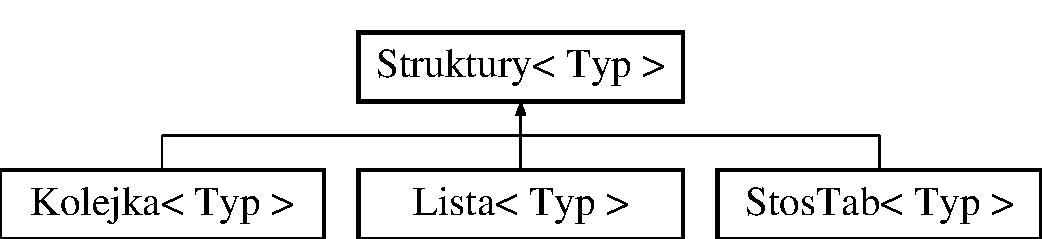
\includegraphics[height=2.000000cm]{class_struktury}
\end{center}
\end{figure}
\subsection*{Public Member Functions}
\begin{DoxyCompactItemize}
\item 
virtual void \hyperlink{class_struktury_aac09c019a75dd7bfda2f313733300c4c}{\-\_\-\-Push} (Typ k, unsigned int Pozycja)=0
\begin{DoxyCompactList}\small\item\em Metoda dodajaca kolejny element struktury. \end{DoxyCompactList}\item 
virtual Typ \hyperlink{class_struktury_a536345360bdb841d5462b578fe758b73}{\-\_\-\-Pop} (unsigned int Pozycja)=0
\begin{DoxyCompactList}\small\item\em Metoda usuwajaca element. \end{DoxyCompactList}\item 
virtual unsigned int \hyperlink{class_struktury_a3ed3c70e26cefc242633abc13097acce}{\-\_\-\-Rozmiar} () const =0
\begin{DoxyCompactList}\small\item\em Metoda zwracajaca rozmiar \hyperlink{class_struktury}{Struktury}. \end{DoxyCompactList}\item 
virtual void \hyperlink{class_struktury_a9a4290d332a6a613f92d4d4bfe2577ae}{\-\_\-\-Pokaz} () const =0
\begin{DoxyCompactList}\small\item\em Metoda wyswietlajaca dane. \end{DoxyCompactList}\item 
virtual void \hyperlink{class_struktury_aa85ab98de0f8bb1c257e6d1723d107f5}{\-\_\-\-Zwolnij} ()=0
\begin{DoxyCompactList}\small\item\em Metoda zwalniajaca pamiec. \end{DoxyCompactList}\end{DoxyCompactItemize}


\subsection{Detailed Description}
\subsubsection*{template$<$class Typ$>$class Struktury$<$ Typ $>$}

Modeluje pojecie \hyperlink{class_struktury}{Struktury} danych, klasa bazowa dla Stosu,Kolejki i Listy,zarowno w implemenetacji wskaznikowej jak i tablicowej. 

\subsection{Member Function Documentation}
\hypertarget{class_struktury_a9a4290d332a6a613f92d4d4bfe2577ae}{\index{Struktury@{Struktury}!\-\_\-\-Pokaz@{\-\_\-\-Pokaz}}
\index{\-\_\-\-Pokaz@{\-\_\-\-Pokaz}!Struktury@{Struktury}}
\subsubsection[{\-\_\-\-Pokaz}]{\setlength{\rightskip}{0pt plus 5cm}template$<$class Typ $>$ virtual void {\bf Struktury}$<$ Typ $>$\-::\-\_\-\-Pokaz (
\begin{DoxyParamCaption}
{}
\end{DoxyParamCaption}
) const\hspace{0.3cm}{\ttfamily [pure virtual]}}}\label{class_struktury_a9a4290d332a6a613f92d4d4bfe2577ae}


Metoda wyswietlajaca dane. 

Metoda ma za zadanie wyswietlic wszytskie dane nalezace do struktury 

Implemented in \hyperlink{class_lista_abae4fe58b5a4225b0df8d98caa65db75}{Lista$<$ Typ $>$}, \hyperlink{class_kolejka_a47121a1d8dd1b45bcf5411ab2d5bc099}{Kolejka$<$ Typ $>$}, and \hyperlink{class_stos_tab_a1b3c30902f28bf819ea5864c85ebede9}{Stos\-Tab$<$ Typ $>$}.

\hypertarget{class_struktury_a536345360bdb841d5462b578fe758b73}{\index{Struktury@{Struktury}!\-\_\-\-Pop@{\-\_\-\-Pop}}
\index{\-\_\-\-Pop@{\-\_\-\-Pop}!Struktury@{Struktury}}
\subsubsection[{\-\_\-\-Pop}]{\setlength{\rightskip}{0pt plus 5cm}template$<$class Typ $>$ virtual Typ {\bf Struktury}$<$ Typ $>$\-::\-\_\-\-Pop (
\begin{DoxyParamCaption}
\item[{unsigned int}]{Pozycja}
\end{DoxyParamCaption}
)\hspace{0.3cm}{\ttfamily [pure virtual]}}}\label{class_struktury_a536345360bdb841d5462b578fe758b73}


Metoda usuwajaca element. 

Metoda ma za zadanie usunac element i w zaleznosci od implementowanej struktury bedzie to usuwany element usuwany z poczatk,końca lub w przypadku listy z dowolnego jej miejsca 
\begin{DoxyParams}[1]{Parameters}
\mbox{\tt in}  & {\em Pozycja} & -\/ Numer elementu ,ktory zostanie dodany. Argument ma znaczenie tylko w przypadku listy i domyślnie jest ustawiony, tak aby element był dodawany zawsze na poczatku listy \\
\hline
\end{DoxyParams}
\begin{DoxyReturn}{Returns}
Zwraca wartosc elementu z odpowiedniego dla wybranej struktury miejsca 
\end{DoxyReturn}


Implemented in \hyperlink{class_kolejka_ab26939041331d337b398819e3cc4443f}{Kolejka$<$ Typ $>$}, \hyperlink{class_lista_a515f4dd7a4ffdfb2fdc12a5fa28e97a4}{Lista$<$ Typ $>$}, and \hyperlink{class_stos_tab_a43e5e031570e69dc27fc11feca969645}{Stos\-Tab$<$ Typ $>$}.

\hypertarget{class_struktury_aac09c019a75dd7bfda2f313733300c4c}{\index{Struktury@{Struktury}!\-\_\-\-Push@{\-\_\-\-Push}}
\index{\-\_\-\-Push@{\-\_\-\-Push}!Struktury@{Struktury}}
\subsubsection[{\-\_\-\-Push}]{\setlength{\rightskip}{0pt plus 5cm}template$<$class Typ $>$ virtual void {\bf Struktury}$<$ Typ $>$\-::\-\_\-\-Push (
\begin{DoxyParamCaption}
\item[{Typ}]{k, }
\item[{unsigned int}]{Pozycja}
\end{DoxyParamCaption}
)\hspace{0.3cm}{\ttfamily [pure virtual]}}}\label{class_struktury_aac09c019a75dd7bfda2f313733300c4c}


Metoda dodajaca kolejny element struktury. 

Metoda ma za zadanie dodac kolejny element do naszej struktury oraz zapisac w nim odpowiednia wartosc.\-W zaleznosci od implementowanej struktury element bedzie dodawany na poczatku lub na koncu struktury danych.


\begin{DoxyParams}[1]{Parameters}
\mbox{\tt in}  & {\em k} & -\/ wartosc typu calkowitnego, ktora bedzie umieszona w strukturze \\
\hline
\end{DoxyParams}


Implemented in \hyperlink{class_stos_tab_a73c95fc8151510c21c5567e85296ea31}{Stos\-Tab$<$ Typ $>$}, \hyperlink{class_kolejka_a215bd2ca4b5db7ec861dfc78ee072858}{Kolejka$<$ Typ $>$}, and \hyperlink{class_lista_a5969ea939160694d8eea3cff3ac34cb8}{Lista$<$ Typ $>$}.

\hypertarget{class_struktury_a3ed3c70e26cefc242633abc13097acce}{\index{Struktury@{Struktury}!\-\_\-\-Rozmiar@{\-\_\-\-Rozmiar}}
\index{\-\_\-\-Rozmiar@{\-\_\-\-Rozmiar}!Struktury@{Struktury}}
\subsubsection[{\-\_\-\-Rozmiar}]{\setlength{\rightskip}{0pt plus 5cm}template$<$class Typ $>$ virtual unsigned int {\bf Struktury}$<$ Typ $>$\-::\-\_\-\-Rozmiar (
\begin{DoxyParamCaption}
{}
\end{DoxyParamCaption}
) const\hspace{0.3cm}{\ttfamily [pure virtual]}}}\label{class_struktury_a3ed3c70e26cefc242633abc13097acce}


Metoda zwracajaca rozmiar \hyperlink{class_struktury}{Struktury}. 

Metoda ma zadanie zwrocic bierzaca liczbe elementow nalezacych do danej struktury \begin{DoxyReturn}{Returns}
-\/ Bierzaca liczba elementow \hyperlink{class_struktury}{Struktury} danych 
\end{DoxyReturn}


Implemented in \hyperlink{class_kolejka_ae76fad7ebe4fbc2bb7900e129a3677bc}{Kolejka$<$ Typ $>$}, \hyperlink{class_stos_tab_a51b2da61d6c4c2085646b84395c2d3c0}{Stos\-Tab$<$ Typ $>$}, and \hyperlink{class_lista_a4fb94c2a9d576a4a32acd1e63f339d38}{Lista$<$ Typ $>$}.

\hypertarget{class_struktury_aa85ab98de0f8bb1c257e6d1723d107f5}{\index{Struktury@{Struktury}!\-\_\-\-Zwolnij@{\-\_\-\-Zwolnij}}
\index{\-\_\-\-Zwolnij@{\-\_\-\-Zwolnij}!Struktury@{Struktury}}
\subsubsection[{\-\_\-\-Zwolnij}]{\setlength{\rightskip}{0pt plus 5cm}template$<$class Typ $>$ virtual void {\bf Struktury}$<$ Typ $>$\-::\-\_\-\-Zwolnij (
\begin{DoxyParamCaption}
{}
\end{DoxyParamCaption}
)\hspace{0.3cm}{\ttfamily [pure virtual]}}}\label{class_struktury_aa85ab98de0f8bb1c257e6d1723d107f5}


Metoda zwalniajaca pamiec. 

Metoda ma za zadanie zwolnic pamiec uzywana przy zapelnienianiu danej struktry danymi 

Implemented in \hyperlink{class_kolejka_a607af93211b5e5e31123c633e1f1fcf2}{Kolejka$<$ Typ $>$}, \hyperlink{class_lista_a3ff3e2f58bd3b1d1b11f9ad68948a321}{Lista$<$ Typ $>$}, and \hyperlink{class_stos_tab_aec0cb259c6f044fa7d3b367dc1baca5c}{Stos\-Tab$<$ Typ $>$}.



The documentation for this class was generated from the following file\-:\begin{DoxyCompactItemize}
\item 
/home/bartolomeo/209255/prj/inc/\hyperlink{_struktury_8hh}{Struktury.\-hh}\end{DoxyCompactItemize}

\hypertarget{class_struktury_benchmark}{\section{Struktury\-Benchmark$<$ Typ $>$ Class Template Reference}
\label{class_struktury_benchmark}\index{Struktury\-Benchmark$<$ Typ $>$@{Struktury\-Benchmark$<$ Typ $>$}}
}


{\ttfamily \#include $<$Struktury\-Benchmark.\-hh$>$}

Inheritance diagram for Struktury\-Benchmark$<$ Typ $>$\-:\begin{figure}[H]
\begin{center}
\leavevmode
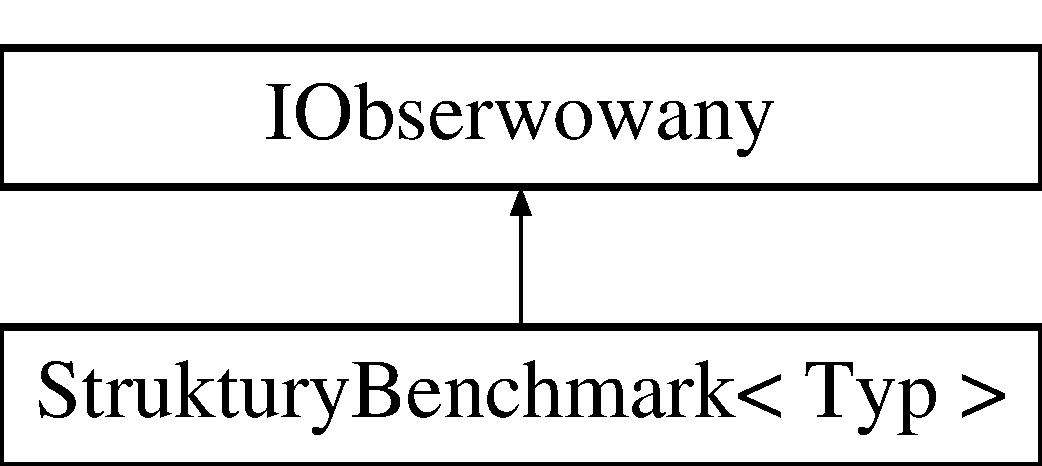
\includegraphics[height=2.000000cm]{class_struktury_benchmark}
\end{center}
\end{figure}
\subsection*{Public Member Functions}
\begin{DoxyCompactItemize}
\item 
\hyperlink{class_struktury_benchmark_a76f71aa0d0ae63409b37cc021a81f2ed}{Struktury\-Benchmark} ()
\item 
virtual \hyperlink{class_struktury_benchmark_a0bb33b43ae5218a09aadf90594d27e75}{$\sim$\-Struktury\-Benchmark} ()
\item 
\hyperlink{class_struktury_benchmark_a044ec90659469fc79e43593d3f6dc442}{Struktury\-Benchmark} (const unsigned int Proby, const unsigned int Powt, const unsigned int $\ast$Rozmiary)
\begin{DoxyCompactList}\small\item\em Konstruktor obiektu. \end{DoxyCompactList}\item 
void \hyperlink{class_struktury_benchmark_a523fc1ac9a7a80dc7182d1a8edf845ec}{\-\_\-\-Wykonaj\-Test} (\hyperlink{class_itest}{Itest} \&W, unsigned int n)
\begin{DoxyCompactList}\small\item\em Metoda inicjalizujaca test. \end{DoxyCompactList}\item 
void \hyperlink{class_struktury_benchmark_a63247cc5616565e429f5abd09d887630}{\-\_\-\-Dodaj\-Obserwator} (\hyperlink{class_i_obserwator}{I\-Obserwator} $\ast$O)
\begin{DoxyCompactList}\small\item\em Metoda dodajaca obserwator. \end{DoxyCompactList}\item 
void \hyperlink{class_struktury_benchmark_af08fe671ed7528428ffcb8a4daf65197}{\-\_\-\-Usun\-Obserwator} (\hyperlink{class_i_obserwator}{I\-Obserwator} $\ast$O)
\begin{DoxyCompactList}\small\item\em Metoda usuwajaca obserwator. \end{DoxyCompactList}\end{DoxyCompactItemize}
\subsection*{Private Member Functions}
\begin{DoxyCompactItemize}
\item 
void \hyperlink{class_struktury_benchmark_af5aa09efcf9a1727e0868930b97ede49}{\-\_\-\-Powiadom\-Obserwatorow} ()
\begin{DoxyCompactList}\small\item\em Metoda wykonujaca test dla odpowiedniej struktury. \end{DoxyCompactList}\end{DoxyCompactItemize}
\subsection*{Private Attributes}
\begin{DoxyCompactItemize}
\item 
std\-::list$<$ \hyperlink{class_i_obserwator}{I\-Obserwator} $\ast$ $>$ \hyperlink{class_struktury_benchmark_a5c96eb86dfccdad59d41d478ca8d66c3}{Obserwatorzy}
\begin{DoxyCompactList}\small\item\em Pole \hyperlink{class_struktury_benchmark}{Struktury\-Benchmark}. \end{DoxyCompactList}\item 
unsigned int \hyperlink{class_struktury_benchmark_a5b2aee5eb235c0ad6c56a4871aad6bd3}{\-\_\-\-Ilosc\-Prob}
\begin{DoxyCompactList}\small\item\em Pole \hyperlink{class_struktury_benchmark}{Struktury\-Benchmark}. \end{DoxyCompactList}\item 
unsigned int \hyperlink{class_struktury_benchmark_a49d86123ea73ecc57bc161dcf40fba01}{\-\_\-\-Ilosc\-Powt}
\begin{DoxyCompactList}\small\item\em Pole \hyperlink{class_struktury_benchmark}{Struktury\-Benchmark}. \end{DoxyCompactList}\item 
unsigned int $\ast$ \hyperlink{class_struktury_benchmark_a9077a191d28f29d9b2eba8d4e8f72ce8}{\-\_\-\-Tablica\-Rozmiarow}
\begin{DoxyCompactList}\small\item\em Pole \hyperlink{class_struktury_benchmark}{Struktury\-Benchmark}. \end{DoxyCompactList}\end{DoxyCompactItemize}
\subsection*{Additional Inherited Members}


\subsection{Detailed Description}
\subsubsection*{template$<$class Typ$>$class Struktury\-Benchmark$<$ Typ $>$}

Klasa modeluje pojecie Benchmarku przeznaczonego dla struktur danych przechowujace dane 

\subsection{Constructor \& Destructor Documentation}
\hypertarget{class_struktury_benchmark_a76f71aa0d0ae63409b37cc021a81f2ed}{\index{Struktury\-Benchmark@{Struktury\-Benchmark}!Struktury\-Benchmark@{Struktury\-Benchmark}}
\index{Struktury\-Benchmark@{Struktury\-Benchmark}!StrukturyBenchmark@{Struktury\-Benchmark}}
\subsubsection[{Struktury\-Benchmark}]{\setlength{\rightskip}{0pt plus 5cm}template$<$class Typ $>$ {\bf Struktury\-Benchmark}$<$ Typ $>$\-::{\bf Struktury\-Benchmark} (
\begin{DoxyParamCaption}
{}
\end{DoxyParamCaption}
)\hspace{0.3cm}{\ttfamily [inline]}}}\label{class_struktury_benchmark_a76f71aa0d0ae63409b37cc021a81f2ed}
\hypertarget{class_struktury_benchmark_a0bb33b43ae5218a09aadf90594d27e75}{\index{Struktury\-Benchmark@{Struktury\-Benchmark}!$\sim$\-Struktury\-Benchmark@{$\sim$\-Struktury\-Benchmark}}
\index{$\sim$\-Struktury\-Benchmark@{$\sim$\-Struktury\-Benchmark}!StrukturyBenchmark@{Struktury\-Benchmark}}
\subsubsection[{$\sim$\-Struktury\-Benchmark}]{\setlength{\rightskip}{0pt plus 5cm}template$<$class Typ $>$ virtual {\bf Struktury\-Benchmark}$<$ Typ $>$\-::$\sim${\bf Struktury\-Benchmark} (
\begin{DoxyParamCaption}
{}
\end{DoxyParamCaption}
)\hspace{0.3cm}{\ttfamily [inline]}, {\ttfamily [virtual]}}}\label{class_struktury_benchmark_a0bb33b43ae5218a09aadf90594d27e75}
\hypertarget{class_struktury_benchmark_a044ec90659469fc79e43593d3f6dc442}{\index{Struktury\-Benchmark@{Struktury\-Benchmark}!Struktury\-Benchmark@{Struktury\-Benchmark}}
\index{Struktury\-Benchmark@{Struktury\-Benchmark}!StrukturyBenchmark@{Struktury\-Benchmark}}
\subsubsection[{Struktury\-Benchmark}]{\setlength{\rightskip}{0pt plus 5cm}template$<$class Typ $>$ {\bf Struktury\-Benchmark}$<$ Typ $>$\-::{\bf Struktury\-Benchmark} (
\begin{DoxyParamCaption}
\item[{const unsigned int}]{Proby, }
\item[{const unsigned int}]{Powt, }
\item[{const unsigned int $\ast$}]{Rozmiary}
\end{DoxyParamCaption}
)\hspace{0.3cm}{\ttfamily [inline]}}}\label{class_struktury_benchmark_a044ec90659469fc79e43593d3f6dc442}


Konstruktor obiektu. 



\subsection{Member Function Documentation}
\hypertarget{class_struktury_benchmark_a63247cc5616565e429f5abd09d887630}{\index{Struktury\-Benchmark@{Struktury\-Benchmark}!\-\_\-\-Dodaj\-Obserwator@{\-\_\-\-Dodaj\-Obserwator}}
\index{\-\_\-\-Dodaj\-Obserwator@{\-\_\-\-Dodaj\-Obserwator}!StrukturyBenchmark@{Struktury\-Benchmark}}
\subsubsection[{\-\_\-\-Dodaj\-Obserwator}]{\setlength{\rightskip}{0pt plus 5cm}template$<$class Typ $>$ void {\bf Struktury\-Benchmark}$<$ Typ $>$\-::\-\_\-\-Dodaj\-Obserwator (
\begin{DoxyParamCaption}
\item[{{\bf I\-Obserwator} $\ast$}]{O}
\end{DoxyParamCaption}
)\hspace{0.3cm}{\ttfamily [inline]}, {\ttfamily [virtual]}}}\label{class_struktury_benchmark_a63247cc5616565e429f5abd09d887630}


Metoda dodajaca obserwator. 

Metoda ma za zadanie dodac nowego obserwatora do listy obserwatorow danego obiektu


\begin{DoxyParams}[1]{Parameters}
\mbox{\tt in}  & {\em O} & -\/ wskaznik na dodawany obserwator \\
\hline
\end{DoxyParams}


Implements \hyperlink{class_i_obserwowany_a3e7c49a1b168ed5a3f84bd0c5ae27513}{I\-Obserwowany}.

\hypertarget{class_struktury_benchmark_af5aa09efcf9a1727e0868930b97ede49}{\index{Struktury\-Benchmark@{Struktury\-Benchmark}!\-\_\-\-Powiadom\-Obserwatorow@{\-\_\-\-Powiadom\-Obserwatorow}}
\index{\-\_\-\-Powiadom\-Obserwatorow@{\-\_\-\-Powiadom\-Obserwatorow}!StrukturyBenchmark@{Struktury\-Benchmark}}
\subsubsection[{\-\_\-\-Powiadom\-Obserwatorow}]{\setlength{\rightskip}{0pt plus 5cm}template$<$class Typ $>$ void {\bf Struktury\-Benchmark}$<$ Typ $>$\-::\-\_\-\-Powiadom\-Obserwatorow (
\begin{DoxyParamCaption}
{}
\end{DoxyParamCaption}
)\hspace{0.3cm}{\ttfamily [inline]}, {\ttfamily [private]}, {\ttfamily [virtual]}}}\label{class_struktury_benchmark_af5aa09efcf9a1727e0868930b97ede49}


Metoda wykonujaca test dla odpowiedniej struktury. 

Metoda ma za zadanie wykonac zapelnienie struktury danymi o zadanej w argumencie ilosci 
\begin{DoxyParams}[1]{Parameters}
\mbox{\tt in}  & {\em n} & -\/ ilosc danych ktora zapelnona struktura\\
\hline
\end{DoxyParams}
Metoda informujaca obserwatorow

Metoda ma za zadanie poinformowac wszystkich obserwatorow o zmianach, ktore sa istotne dla nich, jakie zostaly wykonane na obiekcie obserwowanym 

Implements \hyperlink{class_i_obserwowany_addbe1bee0cae92b0c1348b2c6d0b525c}{I\-Obserwowany}.

\hypertarget{class_struktury_benchmark_af08fe671ed7528428ffcb8a4daf65197}{\index{Struktury\-Benchmark@{Struktury\-Benchmark}!\-\_\-\-Usun\-Obserwator@{\-\_\-\-Usun\-Obserwator}}
\index{\-\_\-\-Usun\-Obserwator@{\-\_\-\-Usun\-Obserwator}!StrukturyBenchmark@{Struktury\-Benchmark}}
\subsubsection[{\-\_\-\-Usun\-Obserwator}]{\setlength{\rightskip}{0pt plus 5cm}template$<$class Typ $>$ void {\bf Struktury\-Benchmark}$<$ Typ $>$\-::\-\_\-\-Usun\-Obserwator (
\begin{DoxyParamCaption}
\item[{{\bf I\-Obserwator} $\ast$}]{O}
\end{DoxyParamCaption}
)\hspace{0.3cm}{\ttfamily [inline]}, {\ttfamily [virtual]}}}\label{class_struktury_benchmark_af08fe671ed7528428ffcb8a4daf65197}


Metoda usuwajaca obserwator. 

Metoda ma za zadanei usunac zadanego poprzez argument obserwatora z listy obserwatorow danego obiektu


\begin{DoxyParams}[1]{Parameters}
\mbox{\tt in}  & {\em O} & -\/ wskaznik na obserwator,ktory ma zostac usuniety \\
\hline
\end{DoxyParams}


Implements \hyperlink{class_i_obserwowany_a6e91b84d0502f038d287152a5d860aff}{I\-Obserwowany}.

\hypertarget{class_struktury_benchmark_a523fc1ac9a7a80dc7182d1a8edf845ec}{\index{Struktury\-Benchmark@{Struktury\-Benchmark}!\-\_\-\-Wykonaj\-Test@{\-\_\-\-Wykonaj\-Test}}
\index{\-\_\-\-Wykonaj\-Test@{\-\_\-\-Wykonaj\-Test}!StrukturyBenchmark@{Struktury\-Benchmark}}
\subsubsection[{\-\_\-\-Wykonaj\-Test}]{\setlength{\rightskip}{0pt plus 5cm}template$<$class Typ $>$ void {\bf Struktury\-Benchmark}$<$ Typ $>$\-::\-\_\-\-Wykonaj\-Test (
\begin{DoxyParamCaption}
\item[{{\bf Itest} \&}]{W, }
\item[{unsigned int}]{n}
\end{DoxyParamCaption}
)\hspace{0.3cm}{\ttfamily [inline]}}}\label{class_struktury_benchmark_a523fc1ac9a7a80dc7182d1a8edf845ec}


Metoda inicjalizujaca test. 

Metoda ma za zadanie uruchomic okreslona ilosc razy testowana metode, czas jej wykonania jest zbierany przez klase zewnetrzna 

\subsection{Member Data Documentation}
\hypertarget{class_struktury_benchmark_a49d86123ea73ecc57bc161dcf40fba01}{\index{Struktury\-Benchmark@{Struktury\-Benchmark}!\-\_\-\-Ilosc\-Powt@{\-\_\-\-Ilosc\-Powt}}
\index{\-\_\-\-Ilosc\-Powt@{\-\_\-\-Ilosc\-Powt}!StrukturyBenchmark@{Struktury\-Benchmark}}
\subsubsection[{\-\_\-\-Ilosc\-Powt}]{\setlength{\rightskip}{0pt plus 5cm}template$<$class Typ $>$ unsigned int {\bf Struktury\-Benchmark}$<$ Typ $>$\-::\-\_\-\-Ilosc\-Powt\hspace{0.3cm}{\ttfamily [private]}}}\label{class_struktury_benchmark_a49d86123ea73ecc57bc161dcf40fba01}


Pole \hyperlink{class_struktury_benchmark}{Struktury\-Benchmark}. 

Pole zawiera informacje o ilosci powtorzen jakie maja zosatc wykonane przy tescie \hypertarget{class_struktury_benchmark_a5b2aee5eb235c0ad6c56a4871aad6bd3}{\index{Struktury\-Benchmark@{Struktury\-Benchmark}!\-\_\-\-Ilosc\-Prob@{\-\_\-\-Ilosc\-Prob}}
\index{\-\_\-\-Ilosc\-Prob@{\-\_\-\-Ilosc\-Prob}!StrukturyBenchmark@{Struktury\-Benchmark}}
\subsubsection[{\-\_\-\-Ilosc\-Prob}]{\setlength{\rightskip}{0pt plus 5cm}template$<$class Typ $>$ unsigned int {\bf Struktury\-Benchmark}$<$ Typ $>$\-::\-\_\-\-Ilosc\-Prob\hspace{0.3cm}{\ttfamily [private]}}}\label{class_struktury_benchmark_a5b2aee5eb235c0ad6c56a4871aad6bd3}


Pole \hyperlink{class_struktury_benchmark}{Struktury\-Benchmark}. 

Pole zawiera informacje o ilosci prob jakie zostana wykonane \hypertarget{class_struktury_benchmark_a9077a191d28f29d9b2eba8d4e8f72ce8}{\index{Struktury\-Benchmark@{Struktury\-Benchmark}!\-\_\-\-Tablica\-Rozmiarow@{\-\_\-\-Tablica\-Rozmiarow}}
\index{\-\_\-\-Tablica\-Rozmiarow@{\-\_\-\-Tablica\-Rozmiarow}!StrukturyBenchmark@{Struktury\-Benchmark}}
\subsubsection[{\-\_\-\-Tablica\-Rozmiarow}]{\setlength{\rightskip}{0pt plus 5cm}template$<$class Typ $>$ unsigned int$\ast$ {\bf Struktury\-Benchmark}$<$ Typ $>$\-::\-\_\-\-Tablica\-Rozmiarow\hspace{0.3cm}{\ttfamily [private]}}}\label{class_struktury_benchmark_a9077a191d28f29d9b2eba8d4e8f72ce8}


Pole \hyperlink{class_struktury_benchmark}{Struktury\-Benchmark}. 

Pole zawiera wskaznik przechowujacy informcje dla jakiej ilosci danych maja zostac wykonane testy \hypertarget{class_struktury_benchmark_a5c96eb86dfccdad59d41d478ca8d66c3}{\index{Struktury\-Benchmark@{Struktury\-Benchmark}!Obserwatorzy@{Obserwatorzy}}
\index{Obserwatorzy@{Obserwatorzy}!StrukturyBenchmark@{Struktury\-Benchmark}}
\subsubsection[{Obserwatorzy}]{\setlength{\rightskip}{0pt plus 5cm}template$<$class Typ $>$ std\-::list$<${\bf I\-Obserwator}$\ast$$>$ {\bf Struktury\-Benchmark}$<$ Typ $>$\-::Obserwatorzy\hspace{0.3cm}{\ttfamily [private]}}}\label{class_struktury_benchmark_a5c96eb86dfccdad59d41d478ca8d66c3}


Pole \hyperlink{class_struktury_benchmark}{Struktury\-Benchmark}. 

Pole zawiera liste obserwatorow,ktore obserwuja ten obiekt 

The documentation for this class was generated from the following file\-:\begin{DoxyCompactItemize}
\item 
/home/bartolomeo/209255/prj/inc/\hyperlink{_struktury_benchmark_8hh}{Struktury\-Benchmark.\-hh}\end{DoxyCompactItemize}

\hypertarget{struct_kolejka_1_1_wezel}{\section{Kolejka$<$ Typ $>$\-:\-:Wezel Struct Reference}
\label{struct_kolejka_1_1_wezel}\index{Kolejka$<$ Typ $>$\-::\-Wezel@{Kolejka$<$ Typ $>$\-::\-Wezel}}
}
\subsection*{Public Attributes}
\begin{DoxyCompactItemize}
\item 
\hyperlink{struct_kolejka_1_1_wezel}{Wezel} $\ast$ \hyperlink{struct_kolejka_1_1_wezel_aadaafaa4a81cf0ddb3fe506688f93c03}{\-\_\-\-Nast}
\begin{DoxyCompactList}\small\item\em Pole Wezla Pole bedace wskaznikiem na kolejny element Kolejki. \end{DoxyCompactList}\item 
Typ \hyperlink{struct_kolejka_1_1_wezel_afb3e7fb216cacf18bef1c69c3e38b7f2}{\-\_\-\-Wartosc}
\begin{DoxyCompactList}\small\item\em Pole Wezla Pole przechowuje wartoc typu calkowitego. \end{DoxyCompactList}\end{DoxyCompactItemize}


\subsection{Detailed Description}
\subsubsection*{template$<$class Typ$>$struct Kolejka$<$ Typ $>$\-::\-Wezel}

Klasy \hyperlink{class_kolejka}{Kolejka} Pole modelje pojecie wezla,bedacego podstawa dla implementacji struktury danych w rozwinieciu wskaznikowym 

\subsection{Member Data Documentation}
\hypertarget{struct_kolejka_1_1_wezel_aadaafaa4a81cf0ddb3fe506688f93c03}{\index{Kolejka\-::\-Wezel@{Kolejka\-::\-Wezel}!\-\_\-\-Nast@{\-\_\-\-Nast}}
\index{\-\_\-\-Nast@{\-\_\-\-Nast}!Kolejka::Wezel@{Kolejka\-::\-Wezel}}
\subsubsection[{\-\_\-\-Nast}]{\setlength{\rightskip}{0pt plus 5cm}template$<$class Typ $>$ {\bf Wezel}$\ast$ {\bf Kolejka}$<$ Typ $>$\-::Wezel\-::\-\_\-\-Nast}}\label{struct_kolejka_1_1_wezel_aadaafaa4a81cf0ddb3fe506688f93c03}


Pole Wezla Pole bedace wskaznikiem na kolejny element Kolejki. 

\hypertarget{struct_kolejka_1_1_wezel_afb3e7fb216cacf18bef1c69c3e38b7f2}{\index{Kolejka\-::\-Wezel@{Kolejka\-::\-Wezel}!\-\_\-\-Wartosc@{\-\_\-\-Wartosc}}
\index{\-\_\-\-Wartosc@{\-\_\-\-Wartosc}!Kolejka::Wezel@{Kolejka\-::\-Wezel}}
\subsubsection[{\-\_\-\-Wartosc}]{\setlength{\rightskip}{0pt plus 5cm}template$<$class Typ $>$ Typ {\bf Kolejka}$<$ Typ $>$\-::Wezel\-::\-\_\-\-Wartosc}}\label{struct_kolejka_1_1_wezel_afb3e7fb216cacf18bef1c69c3e38b7f2}


Pole Wezla Pole przechowuje wartoc typu calkowitego. 



The documentation for this struct was generated from the following file\-:\begin{DoxyCompactItemize}
\item 
/home/bartolomeo/209255/prj/inc/\hyperlink{_kolejka_8hh}{Kolejka.\-hh}\end{DoxyCompactItemize}

\hypertarget{struct_lista_1_1_wezel}{\section{Lista$<$ Typ $>$\-:\-:Wezel Struct Reference}
\label{struct_lista_1_1_wezel}\index{Lista$<$ Typ $>$\-::\-Wezel@{Lista$<$ Typ $>$\-::\-Wezel}}
}
\subsection*{Public Attributes}
\begin{DoxyCompactItemize}
\item 
\hyperlink{struct_lista_1_1_wezel}{Wezel} $\ast$ \hyperlink{struct_lista_1_1_wezel_a6f71b34a0536853ccd08a63c69fba79b}{\-\_\-\-Nast}
\begin{DoxyCompactList}\small\item\em Pole Wezla Pole bedace wskaznikiem na kolejny element listy. \end{DoxyCompactList}\item 
Typ \hyperlink{struct_lista_1_1_wezel_a5873e379887a28a814be35810883e743}{\-\_\-\-Wartosc}
\begin{DoxyCompactList}\small\item\em Pole Wezla Pole przechowuje wartoc typu calkowitego. \end{DoxyCompactList}\end{DoxyCompactItemize}


\subsection{Detailed Description}
\subsubsection*{template$<$class Typ$>$struct Lista$<$ Typ $>$\-::\-Wezel}

Klasy lista Pole modelje pojecie wezla,bedacego podstawa dla implementacji struktury danych w rozwinieciu wskaznikowym 

\subsection{Member Data Documentation}
\hypertarget{struct_lista_1_1_wezel_a6f71b34a0536853ccd08a63c69fba79b}{\index{Lista\-::\-Wezel@{Lista\-::\-Wezel}!\-\_\-\-Nast@{\-\_\-\-Nast}}
\index{\-\_\-\-Nast@{\-\_\-\-Nast}!Lista::Wezel@{Lista\-::\-Wezel}}
\subsubsection[{\-\_\-\-Nast}]{\setlength{\rightskip}{0pt plus 5cm}template$<$class Typ $>$ {\bf Wezel}$\ast$ {\bf Lista}$<$ Typ $>$\-::Wezel\-::\-\_\-\-Nast}}\label{struct_lista_1_1_wezel_a6f71b34a0536853ccd08a63c69fba79b}


Pole Wezla Pole bedace wskaznikiem na kolejny element listy. 

\hypertarget{struct_lista_1_1_wezel_a5873e379887a28a814be35810883e743}{\index{Lista\-::\-Wezel@{Lista\-::\-Wezel}!\-\_\-\-Wartosc@{\-\_\-\-Wartosc}}
\index{\-\_\-\-Wartosc@{\-\_\-\-Wartosc}!Lista::Wezel@{Lista\-::\-Wezel}}
\subsubsection[{\-\_\-\-Wartosc}]{\setlength{\rightskip}{0pt plus 5cm}template$<$class Typ $>$ Typ {\bf Lista}$<$ Typ $>$\-::Wezel\-::\-\_\-\-Wartosc}}\label{struct_lista_1_1_wezel_a5873e379887a28a814be35810883e743}


Pole Wezla Pole przechowuje wartoc typu calkowitego. 



The documentation for this struct was generated from the following file\-:\begin{DoxyCompactItemize}
\item 
/home/bartolomeo/209255/prj/inc/\hyperlink{_lista_8hh}{Lista.\-hh}\end{DoxyCompactItemize}

\hypertarget{class_wyniki}{\section{Wyniki Class Reference}
\label{class_wyniki}\index{Wyniki@{Wyniki}}
}


{\ttfamily \#include $<$Wyniki.\-hh$>$}

Inheritance diagram for Wyniki\-:\begin{figure}[H]
\begin{center}
\leavevmode
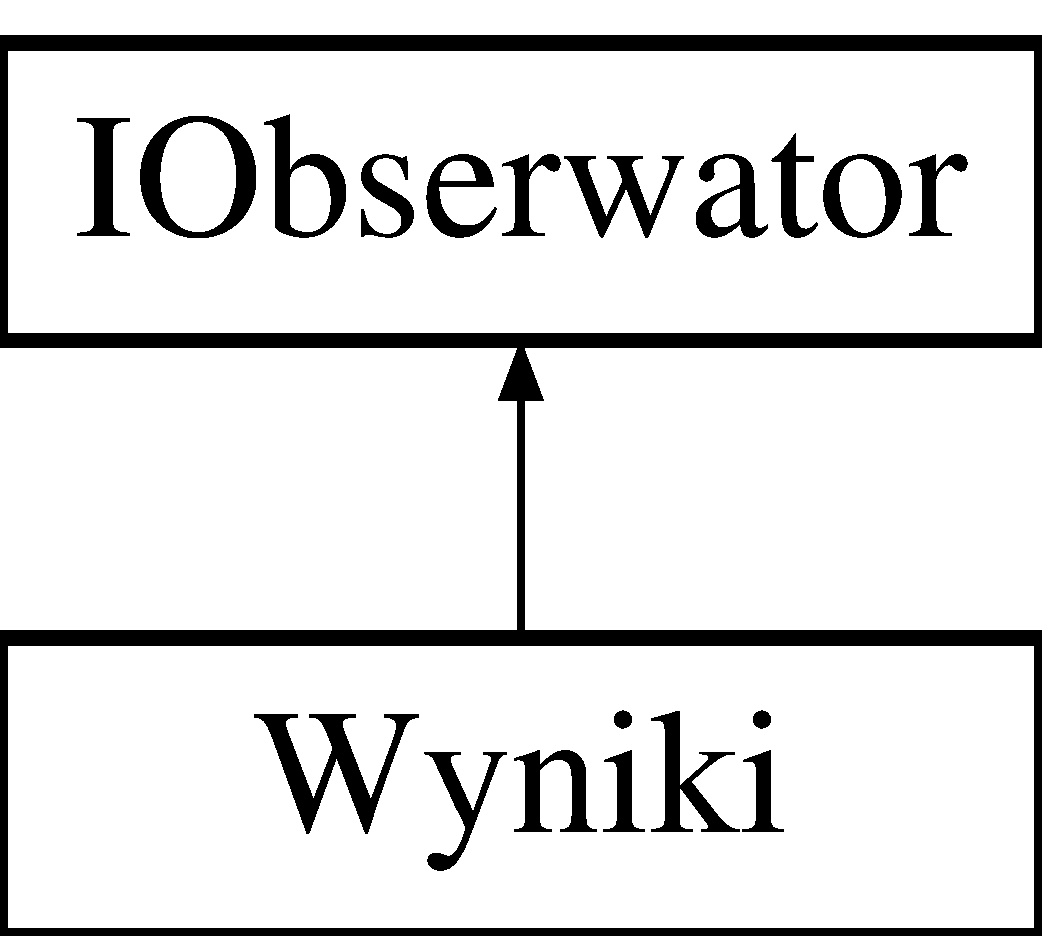
\includegraphics[height=2.000000cm]{class_wyniki}
\end{center}
\end{figure}
\subsection*{Public Member Functions}
\begin{DoxyCompactItemize}
\item 
\hyperlink{class_wyniki_ab5cb499acd382a7e41c294da00648dd4}{Wyniki} ()
\item 
\hyperlink{class_wyniki_a8d370dd59afbd516220a5abbfd5294be}{Wyniki} (const unsigned int Powtorzen, const unsigned int Proby, unsigned int $\ast$Rozmiary)
\item 
virtual \hyperlink{class_wyniki_a0586d35f79012d9961cb4762567357c3}{$\sim$\-Wyniki} ()
\item 
void \hyperlink{class_wyniki_acc5e2bc728f9159a7e244339d84a47c6}{\-\_\-\-Zapisz\-Wyniki} (std\-::string Plik\-Wy) const 
\item 
void \hyperlink{class_wyniki_a4014236438f62cfd90c03de49ea38e5f}{\-\_\-\-Aktualizuj} ()
\begin{DoxyCompactList}\small\item\em Metoda Aktualizujaca stan. \end{DoxyCompactList}\end{DoxyCompactItemize}
\subsection*{Private Attributes}
\begin{DoxyCompactItemize}
\item 
unsigned int \hyperlink{class_wyniki_ac276b321edb9c38043e2b5aba213d847}{\-\_\-\-Ilosc\-Prob}
\item 
unsigned int \hyperlink{class_wyniki_ad207dabc5d9f03c957e1d023276f5548}{\-\_\-\-Ilosc\-Powtorzen}
\item 
unsigned int $\ast$ \hyperlink{class_wyniki_a559a3c3c4374708a493e8636320d9165}{\-\_\-\-Tablica\-Rozmiarow}
\item 
long double $\ast$ \hyperlink{class_wyniki_a6f47caedb424b964c117252febe1f135}{\-\_\-\-Tablica\-Wynikow}
\item 
\hyperlink{class_czasomierz}{Czasomierz} \hyperlink{class_wyniki_ac62ede680255427ef8f51e38e3eddcb9}{Stoper}
\end{DoxyCompactItemize}


\subsection{Constructor \& Destructor Documentation}
\hypertarget{class_wyniki_ab5cb499acd382a7e41c294da00648dd4}{\index{Wyniki@{Wyniki}!Wyniki@{Wyniki}}
\index{Wyniki@{Wyniki}!Wyniki@{Wyniki}}
\subsubsection[{Wyniki}]{\setlength{\rightskip}{0pt plus 5cm}Wyniki\-::\-Wyniki (
\begin{DoxyParamCaption}
{}
\end{DoxyParamCaption}
)}}\label{class_wyniki_ab5cb499acd382a7e41c294da00648dd4}
\hypertarget{class_wyniki_a8d370dd59afbd516220a5abbfd5294be}{\index{Wyniki@{Wyniki}!Wyniki@{Wyniki}}
\index{Wyniki@{Wyniki}!Wyniki@{Wyniki}}
\subsubsection[{Wyniki}]{\setlength{\rightskip}{0pt plus 5cm}Wyniki\-::\-Wyniki (
\begin{DoxyParamCaption}
\item[{const unsigned int}]{Powtorzen, }
\item[{const unsigned int}]{Proby, }
\item[{unsigned int $\ast$}]{Rozmiary}
\end{DoxyParamCaption}
)}}\label{class_wyniki_a8d370dd59afbd516220a5abbfd5294be}
\hypertarget{class_wyniki_a0586d35f79012d9961cb4762567357c3}{\index{Wyniki@{Wyniki}!$\sim$\-Wyniki@{$\sim$\-Wyniki}}
\index{$\sim$\-Wyniki@{$\sim$\-Wyniki}!Wyniki@{Wyniki}}
\subsubsection[{$\sim$\-Wyniki}]{\setlength{\rightskip}{0pt plus 5cm}Wyniki\-::$\sim$\-Wyniki (
\begin{DoxyParamCaption}
{}
\end{DoxyParamCaption}
)\hspace{0.3cm}{\ttfamily [virtual]}}}\label{class_wyniki_a0586d35f79012d9961cb4762567357c3}


\subsection{Member Function Documentation}
\hypertarget{class_wyniki_a4014236438f62cfd90c03de49ea38e5f}{\index{Wyniki@{Wyniki}!\-\_\-\-Aktualizuj@{\-\_\-\-Aktualizuj}}
\index{\-\_\-\-Aktualizuj@{\-\_\-\-Aktualizuj}!Wyniki@{Wyniki}}
\subsubsection[{\-\_\-\-Aktualizuj}]{\setlength{\rightskip}{0pt plus 5cm}void Wyniki\-::\-\_\-\-Aktualizuj (
\begin{DoxyParamCaption}
{}
\end{DoxyParamCaption}
)\hspace{0.3cm}{\ttfamily [virtual]}}}\label{class_wyniki_a4014236438f62cfd90c03de49ea38e5f}


Metoda Aktualizujaca stan. 

Metoda ma za zadanie poinformowac o zmianach w obiekcie ktory jest obserwowany 

Implements \hyperlink{class_i_obserwator_ab01d64a94e127100951aa287d4d2275f}{I\-Obserwator}.

\hypertarget{class_wyniki_acc5e2bc728f9159a7e244339d84a47c6}{\index{Wyniki@{Wyniki}!\-\_\-\-Zapisz\-Wyniki@{\-\_\-\-Zapisz\-Wyniki}}
\index{\-\_\-\-Zapisz\-Wyniki@{\-\_\-\-Zapisz\-Wyniki}!Wyniki@{Wyniki}}
\subsubsection[{\-\_\-\-Zapisz\-Wyniki}]{\setlength{\rightskip}{0pt plus 5cm}void Wyniki\-::\-\_\-\-Zapisz\-Wyniki (
\begin{DoxyParamCaption}
\item[{std\-::string}]{Plik\-Wy}
\end{DoxyParamCaption}
) const}}\label{class_wyniki_acc5e2bc728f9159a7e244339d84a47c6}


\subsection{Member Data Documentation}
\hypertarget{class_wyniki_ad207dabc5d9f03c957e1d023276f5548}{\index{Wyniki@{Wyniki}!\-\_\-\-Ilosc\-Powtorzen@{\-\_\-\-Ilosc\-Powtorzen}}
\index{\-\_\-\-Ilosc\-Powtorzen@{\-\_\-\-Ilosc\-Powtorzen}!Wyniki@{Wyniki}}
\subsubsection[{\-\_\-\-Ilosc\-Powtorzen}]{\setlength{\rightskip}{0pt plus 5cm}unsigned int Wyniki\-::\-\_\-\-Ilosc\-Powtorzen\hspace{0.3cm}{\ttfamily [private]}}}\label{class_wyniki_ad207dabc5d9f03c957e1d023276f5548}
\hypertarget{class_wyniki_ac276b321edb9c38043e2b5aba213d847}{\index{Wyniki@{Wyniki}!\-\_\-\-Ilosc\-Prob@{\-\_\-\-Ilosc\-Prob}}
\index{\-\_\-\-Ilosc\-Prob@{\-\_\-\-Ilosc\-Prob}!Wyniki@{Wyniki}}
\subsubsection[{\-\_\-\-Ilosc\-Prob}]{\setlength{\rightskip}{0pt plus 5cm}unsigned int Wyniki\-::\-\_\-\-Ilosc\-Prob\hspace{0.3cm}{\ttfamily [private]}}}\label{class_wyniki_ac276b321edb9c38043e2b5aba213d847}
\hypertarget{class_wyniki_a559a3c3c4374708a493e8636320d9165}{\index{Wyniki@{Wyniki}!\-\_\-\-Tablica\-Rozmiarow@{\-\_\-\-Tablica\-Rozmiarow}}
\index{\-\_\-\-Tablica\-Rozmiarow@{\-\_\-\-Tablica\-Rozmiarow}!Wyniki@{Wyniki}}
\subsubsection[{\-\_\-\-Tablica\-Rozmiarow}]{\setlength{\rightskip}{0pt plus 5cm}unsigned int$\ast$ Wyniki\-::\-\_\-\-Tablica\-Rozmiarow\hspace{0.3cm}{\ttfamily [private]}}}\label{class_wyniki_a559a3c3c4374708a493e8636320d9165}
\hypertarget{class_wyniki_a6f47caedb424b964c117252febe1f135}{\index{Wyniki@{Wyniki}!\-\_\-\-Tablica\-Wynikow@{\-\_\-\-Tablica\-Wynikow}}
\index{\-\_\-\-Tablica\-Wynikow@{\-\_\-\-Tablica\-Wynikow}!Wyniki@{Wyniki}}
\subsubsection[{\-\_\-\-Tablica\-Wynikow}]{\setlength{\rightskip}{0pt plus 5cm}long double$\ast$ Wyniki\-::\-\_\-\-Tablica\-Wynikow\hspace{0.3cm}{\ttfamily [private]}}}\label{class_wyniki_a6f47caedb424b964c117252febe1f135}
\hypertarget{class_wyniki_ac62ede680255427ef8f51e38e3eddcb9}{\index{Wyniki@{Wyniki}!Stoper@{Stoper}}
\index{Stoper@{Stoper}!Wyniki@{Wyniki}}
\subsubsection[{Stoper}]{\setlength{\rightskip}{0pt plus 5cm}{\bf Czasomierz} Wyniki\-::\-Stoper\hspace{0.3cm}{\ttfamily [private]}}}\label{class_wyniki_ac62ede680255427ef8f51e38e3eddcb9}


The documentation for this class was generated from the following files\-:\begin{DoxyCompactItemize}
\item 
/home/bartolomeo/209255/prj/inc/\hyperlink{_wyniki_8hh}{Wyniki.\-hh}\item 
/home/bartolomeo/209255/prj/src/\hyperlink{_wyniki_8cpp}{Wyniki.\-cpp}\end{DoxyCompactItemize}

\chapter{File Documentation}
\hypertarget{strona-glowna_8dox}{\section{/home/bartolomeo/209255/prj/doc/strona-\/glowna.dox File Reference}
\label{strona-glowna_8dox}\index{/home/bartolomeo/209255/prj/doc/strona-\/glowna.\-dox@{/home/bartolomeo/209255/prj/doc/strona-\/glowna.\-dox}}
}

\hypertarget{_czasomierz_8hh}{\section{/home/bartolomeo/209255/prj/inc/\-Czasomierz.hh File Reference}
\label{_czasomierz_8hh}\index{/home/bartolomeo/209255/prj/inc/\-Czasomierz.\-hh@{/home/bartolomeo/209255/prj/inc/\-Czasomierz.\-hh}}
}
{\ttfamily \#include $<$iostream$>$}\\*
{\ttfamily \#include $<$cstdlib$>$}\\*
{\ttfamily \#include $<$fstream$>$}\\*
{\ttfamily \#include $<$cstring$>$}\\*
\subsection*{Classes}
\begin{DoxyCompactItemize}
\item 
class \hyperlink{class_czasomierz}{Czasomierz}
\begin{DoxyCompactList}\small\item\em Modeluje pojecie Czasomierza. \end{DoxyCompactList}\end{DoxyCompactItemize}

\hypertarget{_graf_8hh}{\section{/home/bartolomeo/209255/prj/inc/\-Graf.hh File Reference}
\label{_graf_8hh}\index{/home/bartolomeo/209255/prj/inc/\-Graf.\-hh@{/home/bartolomeo/209255/prj/inc/\-Graf.\-hh}}
}
{\ttfamily \#include $<$iostream$>$}\\*
{\ttfamily \#include \char`\"{}Kolejka.\-hh\char`\"{}}\\*
{\ttfamily \#include \char`\"{}Lista.\-hh\char`\"{}}\\*
{\ttfamily \#include \char`\"{}Stos\-Tab.\-hh\char`\"{}}\\*
{\ttfamily \#include \char`\"{}Itest.\-hh\char`\"{}}\\*
{\ttfamily \#include \char`\"{}../src/\-Graf.\-cpp\char`\"{}}\\*
\subsection*{Classes}
\begin{DoxyCompactItemize}
\item 
class \hyperlink{class_graf}{Graf$<$ Typ $>$}
\begin{DoxyCompactList}\small\item\em Modeluje pojecie grafu. \end{DoxyCompactList}\end{DoxyCompactItemize}

\hypertarget{_i_obserwator_8hh}{\section{/home/bartolomeo/209255/prj/inc/\-I\-Obserwator.hh File Reference}
\label{_i_obserwator_8hh}\index{/home/bartolomeo/209255/prj/inc/\-I\-Obserwator.\-hh@{/home/bartolomeo/209255/prj/inc/\-I\-Obserwator.\-hh}}
}
\subsection*{Classes}
\begin{DoxyCompactItemize}
\item 
class \hyperlink{class_i_obserwator}{I\-Obserwator}
\begin{DoxyCompactList}\small\item\em Modeluje pojecie interfejsu dla obserwatora. \end{DoxyCompactList}\end{DoxyCompactItemize}

\hypertarget{_i_obserwowany_8hh}{\section{/home/bartolomeo/209255/prj/inc/\-I\-Obserwowany.hh File Reference}
\label{_i_obserwowany_8hh}\index{/home/bartolomeo/209255/prj/inc/\-I\-Obserwowany.\-hh@{/home/bartolomeo/209255/prj/inc/\-I\-Obserwowany.\-hh}}
}
{\ttfamily \#include $<$iostream$>$}\\*
{\ttfamily \#include \char`\"{}I\-Obserwator.\-hh\char`\"{}}\\*
\subsection*{Classes}
\begin{DoxyCompactItemize}
\item 
class \hyperlink{class_i_obserwowany}{I\-Obserwowany}
\begin{DoxyCompactList}\small\item\em Interfejs dla Obserwatora. \end{DoxyCompactList}\end{DoxyCompactItemize}

\hypertarget{_itest_8hh}{\section{/home/bartolomeo/209255/prj/inc/\-Itest.hh File Reference}
\label{_itest_8hh}\index{/home/bartolomeo/209255/prj/inc/\-Itest.\-hh@{/home/bartolomeo/209255/prj/inc/\-Itest.\-hh}}
}
\subsection*{Classes}
\begin{DoxyCompactItemize}
\item 
class \hyperlink{class_itest}{Itest}
\begin{DoxyCompactList}\small\item\em Modeluje pojecie Interfejsu Testujacego. \end{DoxyCompactList}\end{DoxyCompactItemize}

\hypertarget{_kolejka_8hh}{\section{/home/bartolomeo/209255/prj/inc/\-Kolejka.hh File Reference}
\label{_kolejka_8hh}\index{/home/bartolomeo/209255/prj/inc/\-Kolejka.\-hh@{/home/bartolomeo/209255/prj/inc/\-Kolejka.\-hh}}
}
{\ttfamily \#include $<$iostream$>$}\\*
{\ttfamily \#include $<$cstdlib$>$}\\*
{\ttfamily \#include \char`\"{}Struktury.\-hh\char`\"{}}\\*
\subsection*{Classes}
\begin{DoxyCompactItemize}
\item 
class \hyperlink{class_kolejka}{Kolejka$<$ Typ $>$}
\begin{DoxyCompactList}\small\item\em Modeluje pojecie Kolejki. \end{DoxyCompactList}\item 
struct \hyperlink{struct_kolejka_1_1_wezel}{Kolejka$<$ Typ $>$\-::\-Wezel}
\end{DoxyCompactItemize}

\hypertarget{_lista_8hh}{\section{/home/bartolomeo/209255/prj/inc/\-Lista.hh File Reference}
\label{_lista_8hh}\index{/home/bartolomeo/209255/prj/inc/\-Lista.\-hh@{/home/bartolomeo/209255/prj/inc/\-Lista.\-hh}}
}
{\ttfamily \#include $<$iostream$>$}\\*
{\ttfamily \#include \char`\"{}Struktury.\-hh\char`\"{}}\\*
\subsection*{Classes}
\begin{DoxyCompactItemize}
\item 
class \hyperlink{class_lista}{Lista$<$ Typ $>$}
\item 
struct \hyperlink{struct_lista_1_1_wezel}{Lista$<$ Typ $>$\-::\-Wezel}
\end{DoxyCompactItemize}

\hypertarget{_stos_tab_8hh}{\section{/home/bartolomeo/209255/prj/inc/\-Stos\-Tab.hh File Reference}
\label{_stos_tab_8hh}\index{/home/bartolomeo/209255/prj/inc/\-Stos\-Tab.\-hh@{/home/bartolomeo/209255/prj/inc/\-Stos\-Tab.\-hh}}
}
{\ttfamily \#include $<$cstdlib$>$}\\*
{\ttfamily \#include $<$iostream$>$}\\*
{\ttfamily \#include \char`\"{}Struktury.\-hh\char`\"{}}\\*
\subsection*{Classes}
\begin{DoxyCompactItemize}
\item 
class \hyperlink{class_stos_tab}{Stos\-Tab$<$ Typ $>$}
\end{DoxyCompactItemize}

\hypertarget{_struktury_8hh}{\section{/home/bartolomeo/209255/prj/inc/\-Struktury.hh File Reference}
\label{_struktury_8hh}\index{/home/bartolomeo/209255/prj/inc/\-Struktury.\-hh@{/home/bartolomeo/209255/prj/inc/\-Struktury.\-hh}}
}
{\ttfamily \#include $<$iostream$>$}\\*
{\ttfamily \#include $<$cstring$>$}\\*
{\ttfamily \#include $<$sstream$>$}\\*
{\ttfamily \#include $<$fstream$>$}\\*
\subsection*{Classes}
\begin{DoxyCompactItemize}
\item 
class \hyperlink{class_struktury}{Struktury$<$ Typ $>$}
\begin{DoxyCompactList}\small\item\em Modeluje pojecie \hyperlink{class_struktury}{Struktury} danych, klasa bazowa dla Stosu,Kolejki i Listy,zarowno w implemenetacji wskaznikowej jak i tablicowej. \end{DoxyCompactList}\end{DoxyCompactItemize}

\hypertarget{_struktury_benchmark_8hh}{\section{/home/bartolomeo/209255/prj/inc/\-Struktury\-Benchmark.hh File Reference}
\label{_struktury_benchmark_8hh}\index{/home/bartolomeo/209255/prj/inc/\-Struktury\-Benchmark.\-hh@{/home/bartolomeo/209255/prj/inc/\-Struktury\-Benchmark.\-hh}}
}
{\ttfamily \#include $<$iostream$>$}\\*
{\ttfamily \#include $<$cstdlib$>$}\\*
{\ttfamily \#include $<$fstream$>$}\\*
{\ttfamily \#include $<$cstring$>$}\\*
{\ttfamily \#include $<$list$>$}\\*
{\ttfamily \#include \char`\"{}I\-Obserwowany.\-hh\char`\"{}}\\*
{\ttfamily \#include \char`\"{}Itest.\-hh\char`\"{}}\\*
\subsection*{Classes}
\begin{DoxyCompactItemize}
\item 
class \hyperlink{class_struktury_benchmark}{Struktury\-Benchmark$<$ Typ $>$}
\end{DoxyCompactItemize}

\hypertarget{_wyniki_8hh}{\section{/home/bartolomeo/209255/prj/inc/\-Wyniki.hh File Reference}
\label{_wyniki_8hh}\index{/home/bartolomeo/209255/prj/inc/\-Wyniki.\-hh@{/home/bartolomeo/209255/prj/inc/\-Wyniki.\-hh}}
}
{\ttfamily \#include $<$iostream$>$}\\*
{\ttfamily \#include \char`\"{}I\-Obserwator.\-hh\char`\"{}}\\*
{\ttfamily \#include \char`\"{}Czasomierz.\-hh\char`\"{}}\\*
{\ttfamily \#include $<$fstream$>$}\\*
{\ttfamily \#include $<$cstdlib$>$}\\*
{\ttfamily \#include $<$string$>$}\\*
\subsection*{Classes}
\begin{DoxyCompactItemize}
\item 
class \hyperlink{class_wyniki}{Wyniki}
\end{DoxyCompactItemize}

\hypertarget{_czasomierz_8cpp}{\section{/home/bartolomeo/209255/prj/src/\-Czasomierz.cpp File Reference}
\label{_czasomierz_8cpp}\index{/home/bartolomeo/209255/prj/src/\-Czasomierz.\-cpp@{/home/bartolomeo/209255/prj/src/\-Czasomierz.\-cpp}}
}
{\ttfamily \#include \char`\"{}Czasomierz.\-hh\char`\"{}}\\*

\hypertarget{_graf_8cpp}{\section{/home/bartolomeo/209255/prj/src/\-Graf.cpp File Reference}
\label{_graf_8cpp}\index{/home/bartolomeo/209255/prj/src/\-Graf.\-cpp@{/home/bartolomeo/209255/prj/src/\-Graf.\-cpp}}
}

\hypertarget{_main_8cpp}{\section{/home/bartolomeo/209255/prj/src/\-Main.cpp File Reference}
\label{_main_8cpp}\index{/home/bartolomeo/209255/prj/src/\-Main.\-cpp@{/home/bartolomeo/209255/prj/src/\-Main.\-cpp}}
}


funkcja glowna programu  


{\ttfamily \#include \char`\"{}Struktury\-Benchmark.\-hh\char`\"{}}\\*
{\ttfamily \#include \char`\"{}Wyniki.\-hh\char`\"{}}\\*
{\ttfamily \#include \char`\"{}Graf.\-hh\char`\"{}}\\*
\subsection*{Functions}
\begin{DoxyCompactItemize}
\item 
int \hyperlink{_main_8cpp_ae66f6b31b5ad750f1fe042a706a4e3d4}{main} ()
\end{DoxyCompactItemize}
\subsection*{Variables}
\begin{DoxyCompactItemize}
\item 
const unsigned int \hyperlink{_main_8cpp_ab0aeccfb8fc136d141704d2a755f001c}{I\-L\-O\-S\-C\-\_\-\-P\-O\-W} = 10
\item 
const unsigned int \hyperlink{_main_8cpp_aeb2c52ec07363ba976b3a3030bb79bb5}{I\-L\-O\-S\-C\-\_\-\-P\-R\-O\-B} = 7
\end{DoxyCompactItemize}


\subsection{Detailed Description}
funkcja glowna programu 

\subsection{Function Documentation}
\hypertarget{_main_8cpp_ae66f6b31b5ad750f1fe042a706a4e3d4}{\index{Main.\-cpp@{Main.\-cpp}!main@{main}}
\index{main@{main}!Main.cpp@{Main.\-cpp}}
\subsubsection[{main}]{\setlength{\rightskip}{0pt plus 5cm}int main (
\begin{DoxyParamCaption}
{}
\end{DoxyParamCaption}
)}}\label{_main_8cpp_ae66f6b31b5ad750f1fe042a706a4e3d4}


\subsection{Variable Documentation}
\hypertarget{_main_8cpp_ab0aeccfb8fc136d141704d2a755f001c}{\index{Main.\-cpp@{Main.\-cpp}!I\-L\-O\-S\-C\-\_\-\-P\-O\-W@{I\-L\-O\-S\-C\-\_\-\-P\-O\-W}}
\index{I\-L\-O\-S\-C\-\_\-\-P\-O\-W@{I\-L\-O\-S\-C\-\_\-\-P\-O\-W}!Main.cpp@{Main.\-cpp}}
\subsubsection[{I\-L\-O\-S\-C\-\_\-\-P\-O\-W}]{\setlength{\rightskip}{0pt plus 5cm}const unsigned int I\-L\-O\-S\-C\-\_\-\-P\-O\-W = 10}}\label{_main_8cpp_ab0aeccfb8fc136d141704d2a755f001c}
\hypertarget{_main_8cpp_aeb2c52ec07363ba976b3a3030bb79bb5}{\index{Main.\-cpp@{Main.\-cpp}!I\-L\-O\-S\-C\-\_\-\-P\-R\-O\-B@{I\-L\-O\-S\-C\-\_\-\-P\-R\-O\-B}}
\index{I\-L\-O\-S\-C\-\_\-\-P\-R\-O\-B@{I\-L\-O\-S\-C\-\_\-\-P\-R\-O\-B}!Main.cpp@{Main.\-cpp}}
\subsubsection[{I\-L\-O\-S\-C\-\_\-\-P\-R\-O\-B}]{\setlength{\rightskip}{0pt plus 5cm}const unsigned int I\-L\-O\-S\-C\-\_\-\-P\-R\-O\-B = 7}}\label{_main_8cpp_aeb2c52ec07363ba976b3a3030bb79bb5}

\hypertarget{_wyniki_8cpp}{\section{/home/bartolomeo/209255/prj/src/\-Wyniki.cpp File Reference}
\label{_wyniki_8cpp}\index{/home/bartolomeo/209255/prj/src/\-Wyniki.\-cpp@{/home/bartolomeo/209255/prj/src/\-Wyniki.\-cpp}}
}
{\ttfamily \#include \char`\"{}Wyniki.\-hh\char`\"{}}\\*

%--- End generated contents ---

% Index
\newpage
\phantomsection
\addcontentsline{toc}{chapter}{Index}
\printindex

\end{document}
